% ============================================================
%  Compile: pdfLaTeX (two passes for TOC and references)
%  Overleaf: Menu > Compiler > pdfLaTeX (default)
% ============================================================
\documentclass[12pt, a4paper]{report}

% --- Encoding ---
\usepackage[T1]{fontenc}
\usepackage[utf8]{inputenc}

% --- Font: Times New Roman equivalent ---
\usepackage{mathptmx}   % text + math in Times
\usepackage[scaled=0.92]{helvet}  % Helvetica (sans-serif)
\usepackage{courier}              % Courier (monospace)

% --- Language ---
\usepackage[english]{babel}

% --- Page layout ---
\usepackage{geometry}
\geometry{top=2.5cm, bottom=2.5cm, left=3.5cm, right=2cm}

% --- Line spacing ---
\usepackage{setspace}
\onehalfspacing

% --- Tables ---
\usepackage{booktabs}
\usepackage{tabularx}
\usepackage{multirow}
\usepackage{longtable}
\usepackage{array}

% --- Figures ---
\usepackage{graphicx}
\usepackage{float}
\usepackage{caption}
\usepackage{subcaption}

% --- Mathematics ---
\usepackage{amsmath}
\usepackage{amssymb}

% --- Code listing ---
\usepackage{listings}
\usepackage{xcolor}
\lstset{
  basicstyle=\ttfamily\small,
  breaklines=true,
  frame=single,
  backgroundcolor=\color{gray!10},
  keywordstyle=\color{blue},
  commentstyle=\color{green!60!black},
  stringstyle=\color{orange!80!black},
}

% --- Hyperlinks ---
\usepackage{hyperref}
\hypersetup{
  colorlinks=true,
  linkcolor=black,
  citecolor=blue,
  urlcolor=blue
}

% --- Lists ---
\usepackage{enumitem}

% --- Header / Footer ---
\usepackage{fancyhdr}
\pagestyle{fancy}
\fancyhf{}
\fancyhead[R]{\thepage}
\fancyhead[L]{\leftmark}
\renewcommand{\headrulewidth}{0.4pt}

% --- Chapter title format ---
\usepackage{titlesec}
\titleformat{\chapter}[block]
  {\normalfont\Large\bfseries\centering}{CHAPTER \thechapter.}{1em}{}
\titlespacing*{\chapter}{0pt}{20pt}{20pt}

% --- Utility command: placeholder for missing data ---
\newcommand{\placeholder}[1]{\textit{\textcolor{gray}{[#1]}}}

% ============================================================
\begin{document}

% ============================================================
%  TITLE PAGE
% ============================================================
\begin{titlepage}
\centering
\vspace*{1cm}

{\Large\bfseries UNIVERSITY OF SCIENCE AND TECHNOLOGY OF HANOI (USTH)}\\[0.3cm]
{\large\bfseries DEPARTMENT OF ICT}\\[2cm]

\rule{\linewidth}{0.5pt}\\[0.4cm]
{\LARGE\bfseries AUTOMATED CUSTOMER INTERACTION\\[0.3cm]
AND ORDER MANAGEMENT\\[0.3cm]
IN ONLINE RETAIL}\\[0.4cm]
\rule{\linewidth}{0.5pt}\\[1.5cm]

{\large\bfseries GRADUATION THESIS}\\[2cm]

\begin{flushleft}
{\large
\textbf{Student:} NGUYEN DUC THANH \\[0.3cm]
\textbf{Student ID:} 23BI14406 \\[0.3cm]
\textbf{Supervisor:} DR. DOAN NHAT QUANG \\[0.3cm]
\textbf{Program:} Data Science \\[0.3cm]
}
\end{flushleft}

\vfill
{\large Ha Noi, 06/2026}
\end{titlepage}

\tableofcontents
\listoftables
\listoffigures

\chapter*{List of Abbreviations}
\addcontentsline{toc}{chapter}{List of Abbreviations}

\begin{tabular}{ll}
\toprule
\textbf{Abbreviation} & \textbf{Full form} \\
\midrule
NLP   & Natural Language Processing \\
NLU   & Natural Language Understanding \\
NER   & Named Entity Recognition \\
BERT  & Bidirectional Encoder Representations from Transformers \\
LLM   & Large Language Model \\
RAG   & Retrieval-Augmented Generation \\
TF-IDF & Term Frequency--Inverse Document Frequency \\
SVM   & Support Vector Machine \\
API   & Application Programming Interface \\
BIO   & Beginning, Inside, Outside (NER tagging scheme) \\
EDA   & Exploratory Data Analysis \\
GPU   & Graphics Processing Unit \\
JSON  & JavaScript Object Notation \\
HTTP  & Hypertext Transfer Protocol \\
\bottomrule
\end{tabular}

% ============================================================
%  CHAPTER 1 — INTRODUCTION
% ============================================================
\chapter{Introduction}

\section{Background and Motivation}

E-commerce in Vietnam has grown rapidly in recent years,
particularly in the retail sector for toy building sets and LEGO models.
Handling customer inquiries through chat channels (Facebook Messenger, Zalo, websites)
requires customer service teams to respond quickly and accurately ---
from product consultation and stock checking to order confirmation and payment support.

The rise of Large Language Models (LLMs) such as GPT-4 and Gemini has opened up
the possibility of building next-generation chatbots capable of handling natural
conversation without programming explicit rules for each case. However,
every LLM response consumes hundreds to thousands of API tokens,
leading to operating costs that scale linearly with user traffic.
For small and medium-sized businesses, this represents a significant barrier.

An alternative approach is to build a Natural Language Understanding (NLU) system
based on small language models fine-tuned for specific tasks,
combined with a rule-based pipeline to control the conversation flow.
This approach incurs near-zero inference cost once trained and deployed,
but requires greater investment during development and data annotation.

This thesis builds both systems running in parallel on the same interface,
with the goal of objectively measuring and comparing operating costs,
response latency, and conversation quality under real-world conditions.

\section{Research Objectives and Questions}

This thesis addresses three main research questions:

\begin{enumerate}
  \item \textbf{RQ1:} Can a small NLU model (PhoBERT for intent classification +
        ViSoBERT for entity recognition) combined with a rule-based pipeline
        effectively handle real Vietnamese sales conversations?
  \item \textbf{RQ2:} How large is the difference in operating cost
        (API tokens, latency, estimated expense) between the hybrid NLU + rule-based
        system and a full-LLM chatbot?
  \item \textbf{RQ3:} Does explicit text normalization (teen-code $\rightarrow$ standard)
        combined with word segmentation help PhoBERT compete with ViSoBERT
        on informal Vietnamese chat data?
\end{enumerate}

\section{Scope and Limitations}

\begin{itemize}
  \item \textbf{Language:} Informal Vietnamese with code-switching
        (brand names: LEGO, Ferrari, Porsche, Technic, etc.).
  \item \textbf{Domain:} Online LEGO retail shop --- product consultation,
        order placement, and payment support.
  \item \textbf{Data:} Real chat history from the shop;
        product catalog of 11,362 records from 2010--2026.
  \item \textbf{Comparison scope:} NLU accuracy (Macro-F1, Micro-F1),
        response latency (ms), and API token cost.
\end{itemize}

\section{Contributions}

\begin{itemize}
  \item Construction of a Vietnamese chat dataset annotated with
        32 intent classes and 13 entity types for the e-commerce toy domain.
  \item Comparison of four intent classification approaches
        (SVM, ViSoBERT, PhoBERT + normalization, XLM-RoBERTa),
        achieving Macro-F1 = 0.9022 on the test set.
  \item Quantitative analysis of operating costs between the hybrid NLU + rule-based
        system and the full-LLM chatbot under real-world conditions.
  \item Development of a hybrid RAG pipeline (keyword matching + semantic search)
        optimized for a large product catalog ($\sim$11K records).
\end{itemize}

\section{Report Structure}

This report is organized into eight chapters:
Chapter 2 presents specific project objectives;
Chapter 3 covers the theoretical background;
Chapter 4 analyzes data and preprocessing;
Chapters 5 and 6 are the core --- presenting intent classification experiments
(including the detailed workflow and architecture of Approach 3)
and named entity recognition with evaluation results, respectively;
Chapter 7 describes the chatbot system architecture and use cases;
Chapter 8 provides a comparative evaluation of both modes;
and the Conclusion summarizes findings and suggests future directions.

% ============================================================
%  CHAPTER 2 — OBJECTIVES
% ============================================================
\chapter{Objectives}

\section{Desired Features}

This thesis builds a complete Vietnamese sales chatbot system
with the following core features:

\begin{itemize}
  \item \textbf{FEATURE 1 --- Intent Classification:}
        Automatically classify customer intent into 32 classes (multi-label)
        from informal Vietnamese messages.
        \begin{itemize}
          \item SUB-FEATURE 1.1: Text normalization (teen-code normalization)
          \item SUB-FEATURE 1.2: Word segmentation
          \item SUB-FEATURE 1.3: Fine-tune PhoBERT with per-class threshold tuning
        \end{itemize}

  \item \textbf{FEATURE 2 --- Named Entity Recognition:}
        Extract 13 entity types from messages
        (customer name, phone number, address, product name, budget, delivery time, etc.).

  \item \textbf{FEATURE 3 --- Hybrid Chatbot Pipeline (NLU + Rule-based):}
        End-to-end order conversation processing through a 14-branch priority pipeline
        and an order lifecycle state machine.
        \begin{itemize}
          \item SUB-FEATURE 3.1: Product search and top-3 recommendation
          \item SUB-FEATURE 3.2: Order placement flow (slot-filling)
          \item SUB-FEATURE 3.3: Payment confirmation (bank transfer / COD)
          \item SUB-FEATURE 3.4: Order persistence to database (SQLite)
        \end{itemize}

  \item \textbf{FEATURE 4 --- Full-LLM Baseline (cost comparison):}
        Deploy a Gemini 2.5 Flash Lite + hybrid RAG retrieval chatbot
        running in parallel for token/latency cost comparison against FEATURE 3.

  \item \textbf{FEATURE 5 --- Metrics \& Logging:}
        Per-turn logging (JSONL) and a live \texttt{/metrics} dashboard comparing
        latency, tokens, and estimated cost (VND) between both modes.
\end{itemize}

\section{Expected Outcome}

\begin{table}[H]
\centering
\caption{Expected outcome targets}
\label{tab:expected_outcome}
\begin{tabular}{llc}
\toprule
\textbf{Component} & \textbf{Metric} & \textbf{Target} \\
\midrule
Intent Classification & Test Macro-F1           & $\geq 0.85$ \\
NER                   & Test Micro-F1           & $\geq 0.65$ \\
Hybrid chatbot        & Average latency         & $\leq 500$\,ms \\
Full-LLM baseline     & Token usage             & Fully measured and logged \\
Cost comparison       & Cost ratio Hybrid / LLM & $< 0.01$ \\
\bottomrule
\end{tabular}
\end{table}

% ============================================================
%  CHAPTER 3 — THEORETICAL BACKGROUND
% ============================================================
\chapter{Theoretical Background}

\section{Characteristics of Vietnamese in Social Media Text}

\subsection{Challenges of Vietnamese Chat Text}

Vietnamese in an e-commerce chat environment exhibits several characteristics
that differ substantially from formal text (news articles, academic documents):

\begin{itemize}
  \item \textbf{Teen-code and abbreviations:} Users abbreviate common words
        to save time. For example: \texttt{k}/\texttt{ko} = ``kh\^ong'' (no/not),
        \texttt{dc}/\texttt{dc} = ``du\textit{o}c'' (okay),
        \texttt{sop} = ``shop'', \texttt{ck} = ``chuyen khoan'' (bank transfer).
  \item \textbf{Code-switching:} Brand and product names are typically in English
        (\texttt{lego}, \texttt{ferrari}, \texttt{technic})
        and appear mixed within Vietnamese sentences.
  \item \textbf{Very short sentences:} Most messages contain only 1--15 words,
        lacking clear syntactic context.
  \item \textbf{Repeated emotional characters:} ``oiiii'', ``okkkk'', ``shoppp oiiii''.
\end{itemize}

\subsection{Vietnamese Word Segmentation}

Unlike English, written Vietnamese does not use spaces between syllables
within a compound word (e.g., ``ha noi'', ``chuyen khoan'', ``san pham'').
PhoBERT was pre-trained on word-segmented text;
feeding unsegmented input therefore creates a train-inference register mismatch.
The \textbf{underthesea} library \cite{underthesea} performs word segmentation
in pure Python without a Java dependency, making it suitable for production pipelines.

\section{Transformer Architecture and BERT}

\subsection{Self-Attention Mechanism}

The Transformer \cite{vaswani2017attention} uses self-attention to model
relationships between all token pairs in the input sequence
regardless of their positional distance:

\begin{equation}
  \text{Attention}(Q, K, V) = \text{softmax}\!\left(\frac{QK^T}{\sqrt{d_k}}\right)V
\end{equation}

where $Q$, $K$, $V$ are Query, Key, and Value matrices linearly projected
from the input representation, and $d_k$ is the dimensionality of the Key vector.

\subsection{BERT and Fine-tuning Strategy}

BERT \cite{devlin2019bert} applies two pre-training tasks
(Masked Language Modeling and Next Sentence Prediction) on large-scale text
to learn general semantic representations. When fine-tuned for classification,
the \texttt{[CLS]} vector at the final layer is fed into a linear classification head:

\begin{equation}
  \hat{y} = \sigma(W \cdot h_{[\text{CLS}]} + b)
\end{equation}

All parameters (backbone + classification head) are updated jointly
with a small learning rate (typically $2 \times 10^{-5}$).

\section{Vietnamese BERT Variants}

\subsection{PhoBERT}

PhoBERT \cite{nguyen2020phobert} is a BERT model pre-trained on approximately
20 GB of formal Vietnamese text (online news, Wikipedia),
using a BPE tokenizer with a 64K-token vocabulary.
Input text must be word-segmented before feeding (via VnCoreNLP or underthesea)
to match the register of the pre-training corpus.

\subsection{ViSoBERT}

ViSoBERT \cite{visobert2023} is a BERT model pre-trained on Vietnamese social media text
(Facebook, Twitter, YouTube comments),
covering teen-code, emojis, and common code-switching.
ViSoBERT does not require word segmentation and processes raw text directly.

\subsection{XLM-RoBERTa}

XLM-RoBERTa \cite{conneau2020xlmr} was pre-trained on a 100-language corpus
($\sim$2.5 TB of text) including both Vietnamese and English.
It is the only model in our comparison suite with strong representations
for both languages appearing in the chat data
(Vietnamese and English brand names).

\section{Multi-label Text Classification}

In multi-label classification, each sample may belong to multiple classes simultaneously.
Instead of softmax (single-label), each class is predicted independently with sigmoid:

\begin{equation}
  \hat{y}_i = \sigma(z_i) = \frac{1}{1 + e^{-z_i}}, \quad i = 1,\ldots,C
\end{equation}

The loss function is Binary Cross-Entropy with positive-class weights
(\texttt{pos\_weight}) to address class imbalance:

\begin{equation}
  \mathcal{L} = -\frac{1}{C}\sum_{i=1}^{C}
  \left[ w_i \cdot y_i \log\hat{y}_i + (1 - y_i)\log(1-\hat{y}_i) \right]
\end{equation}

where $w_i = (N - n_i) / n_i$, with $N$ being the total number of samples
and $n_i$ the number of positive samples for class $i$.

\section{Named Entity Recognition (NER)}

\subsection{BIO Tagging}

The BIO scheme assigns a label to each token:
B-\textit{TYPE} (first token of an entity), I-\textit{TYPE}
(continuation token within the same entity), O (outside any entity).
Example:

\begin{center}
\texttt{cho / minh / 2 / bo / Porsche / tam / 900k}\\
\texttt{O \quad O \quad B-QUANTITY \quad I-QUANTITY \quad B-PRODUCT\_NAME \quad O \quad B-MAX\_BUDGET}
\end{center}

\subsection{Token Classification with BERT}

Instead of using the \texttt{[CLS]} vector, the NER model uses
each token's hidden representation $h_t$ to predict the BIO label:

\begin{equation}
  \hat{y}_t = \text{softmax}(W \cdot h_t + b)
\end{equation}

Since BERT uses subword tokenization (BPE), a single word may be split into
multiple subwords. The \textbf{first-subword} aggregation strategy is used:
the word's label is determined by its first subword;
subsequent subwords of the same word are discarded during result aggregation.

\section{Large Language Models and Gemini}

Large language models (LLMs) \cite{google2024gemini} are trained on hundreds
of billions of tokens and can perform diverse language tasks through prompting
alone, without task-specific fine-tuning.

In this thesis, \textbf{Gemini 2.5 Flash Lite} is used as the full-LLM baseline.
The model receives a system instruction, product context (from RAG),
and the last 10 turns of conversation history, then generates a natural response.
Its main drawback is that API cost scales directly with the number of tokens
processed per turn.

\section{Retrieval-Augmented Generation (RAG)}

RAG \cite{lewis2020rag} combines information retrieval with language generation.
The pipeline consists of two steps:

\begin{enumerate}
  \item \textbf{Retrieval:} Embed the query as a vector;
        perform cosine similarity search on a pre-built embedding index.
  \item \textbf{Generation:} The LLM receives the retrieved product context
        along with the user query to generate a response.
\end{enumerate}

This thesis extends basic RAG with \textbf{hybrid retrieval}:
Latin tokens $\geq$ 4 characters in the query (brand names: \texttt{porsche}, \texttt{ferrari})
are extracted for keyword matching first,
then the remaining top-$k$ slots are filled by cosine search.
This ensures that specific brand names always appear in the context
even when cosine similarity is diluted by generic terms.

\section{Slot-Filling Dialogue Systems}

Task-oriented chatbots operate on three layers:
intent recognition, entity extraction, and slot update in the dialogue state.
At each turn, the system inspects the current \textit{dialogue state}
to decide the next action (request more information, confirm, or execute a task).
This decision mechanism is modeled as a \textit{state machine}.

% ============================================================
%  CHAPTER 4 — DATA
% ============================================================
\chapter{Data: Collection, Analysis and Preprocessing}

\section{Data Collection}

\subsection{Dialogue Data --- Intent Classification}

The intent classification dataset was built using a hybrid collection strategy
that balances authenticity and scale:

\begin{itemize}
  \item \textbf{40\% real data:} Messages exported from the shop's actual
        Meta Instagram chat history (The Lego Shop).
        Data was anonymized (personal customer information removed)
        and manually annotated on \textbf{Doccano} \cite{doccano2018} ---
        an open-source text annotation platform with a web interface,
        user role management, and direct JSONL export.
        Each message was assigned one or more labels from the set of 32 intent classes
        based on the shop's business analysis.

  \item \textbf{60\% synthetic data:} The remaining samples were generated
        by an LLM (Gemini 2.5 Flash Lite) per intent class
        to supplement rare classes (fewer than 50 real samples)
        without additional manual annotation effort.
        The LLM was instructed to generate messages in the style of
        informal Vietnamese chat (teen-code, short sentences, code-switching)
        to preserve the language distribution of the real data.
\end{itemize}

\subsection{Dialogue Data --- NER Annotation}
\label{subsec:ner_annotation}

NER annotation requires pinpointing exact character offsets for each entity span.
This thesis adopts a two-phase hybrid approach combining manual and LLM-assisted annotation:

\begin{enumerate}
  \item \textbf{Phase 1 --- Manual annotation (20\%):}
        A subset is fully annotated by hand to ensure quality and label consistency.
        This subset serves both as \textit{ground truth} for evaluation
        and as \textit{few-shot examples} for the next phase.

  \item \textbf{Phase 2 --- LLM-assisted annotation (80\%):}
        The remaining data is annotated automatically using Gemini 2.5 Flash Lite.
        Each annotation script embeds examples from Phase~1 directly in its prompt
        to guide the LLM on label boundaries and output format
        (JSON array \texttt{[\{"label": "...", "text": "exact substring"\}]}).
\end{enumerate}

\paragraph{Automatic annotation pipeline structure (Phase 2)}
The NER annotation scripts share a common processing architecture:

\begin{enumerate}
  \item \textbf{Few-shot prompt:} Defines target label set and embeds real examples
        from the manually annotated set to illustrate ambiguous boundaries
        (e.g., distinguishing ADDRESS from CITY,
        or MIN\_BUDGET from MAX\_BUDGET in a price range).
  \item \textbf{Offset mapping:} The \texttt{find\_spans()} function maps
        entity text to character positions \texttt{(start, end)} in the original sentence
        using \texttt{str.find()}, handling repeated occurrences of the same text.
  \item \textbf{Retry \& Resume:} Automatically retries up to 3 times on API errors
        or invalid JSON; supports checkpoint-based resumption to avoid data loss on interruption.
\end{enumerate}

The results of both phases are merged into a single NER dataset
covering all 13 entity types.

\paragraph{Augmentation script --- \texttt{augment\_ner\_data.py}}
After the first training round, per-entity F1 analysis revealed several entity types
with low performance due to insufficient data.
The script generates targeted synthetic samples specifically for weak entity types
rather than augmenting uniformly:

\begin{table}[H]
\centering
\caption{Targeted NER data augmentation by weak entity type}
\label{tab:ner_augment}
\begin{tabular}{lccl}
\toprule
\textbf{Entity} & \textbf{Original count} & \textbf{After augmentation} & \textbf{Reason} \\
\midrule
\texttt{COMPLEXITY}      & 91  & 200 & F1 = 0.33 (weakest) \\
\texttt{TYPE}            & 106 & 200 & F1 = 0.40 \\
\texttt{PRODUCT\_COLOR}  & 15  & 100 & F1 = 0.55 \\
\texttt{QUANTITY}        & 23  & 100 & Insufficient diverse examples \\
\texttt{MIN\_BUDGET}     & 20  & 100 & Imbalanced vs MAX\_BUDGET \\
\texttt{SHIP\_TIME/DATE} & ---  & +50 & Boundary errors (two labels merged) \\
\texttt{NAME} (lowercase)& ---  & +30 & Insufficient casing diversity \\
\texttt{CITY} (abbreviated)& ---  & +20 & hn, hp, sg, hcm, dn, etc. \\
\midrule
\multicolumn{4}{l}{\textit{Not augmented: \texttt{PRODUCT\_NAME} (574 samples),
\texttt{PHONE} (F1=1.00),}} \\
\multicolumn{4}{l}{\textit{\texttt{ADDRESS} (F1=0.73), \texttt{NAME} (F1=0.95),
\texttt{MAX\_BUDGET} (F1=0.87)}} \\
\bottomrule
\end{tabular}
\end{table}

The remaining 20\% of NER data was manually reviewed to detect LLM annotation errors,
particularly for \texttt{ADDRESS}, which follows diverse Vietnamese address syntax.

\subsection{Product Data}

The product catalog contains \textbf{11,362 records} of LEGO sets from 2010 to 2026,
collected automatically via the \textbf{Rebrickable API} \cite{rebrickable} ---
a community platform providing comprehensive metadata for all released LEGO sets,
including set ID, name, piece count, theme, and sub-theme.
Data was then cleaned and augmented with estimated retail prices for the Vietnamese market
based on USD official prices with a conversion rate.
Each record includes: product ID, name, price (VND), piece count,
theme category (Technic, City, Harry Potter, etc.), and release year.

\section{Exploratory Data Analysis (EDA)}

\subsection{Overall Statistics}

\begin{table}[H]
\centering
\caption{Summary statistics of the dialogue dataset}
\label{tab:data_stats}
\begin{tabular}{lc}
\toprule
\textbf{Metric} & \textbf{Value} \\
\midrule
Total messages               & 4,509 \\
Number of intent classes     & 32 \\
Number of entity types       & 13 \\
Multi-label sample ratio     & 10.6\% \\
Average length (words/msg)   & 7.7 \\
Median length (words/msg)    & 8 \\
Minimum length               & 1 word \\
Maximum length               & 37 words \\
Train / Val / Test split     & 3,605 / 454 / 450 \\
\bottomrule
\end{tabular}
\end{table}

\subsection{Distribution of 32 Intent Classes}

The dataset exhibits significant class imbalance.
The most frequent class (\texttt{give\_product}) represents approximately 10.55\%
of all samples, while the rarest class (\texttt{ask\_find\_product}) accounts for
only 0.94\%.

\begin{table}[H]
\centering
\caption{Selected intent classes and sample counts}
\label{tab:intent_dist}
\begin{tabularx}{\linewidth}{lXc}
\toprule
\textbf{Intent} & \textbf{Description} & \textbf{Count} \\
\midrule
\texttt{give\_product}              & Request to provide product information & 528 \\
\texttt{ask\_product\_price}        & Inquire about product price            & 386 \\
\texttt{ask\_product\_availability} & Inquire about stock availability       & 259 \\
\texttt{other}                      & Out-of-scope request                   & 237 \\
\texttt{ask\_order\_status}         & Inquire about order status             & 230 \\
\texttt{provide\_cus\_inf}          & Provide customer information           & 193 \\
\texttt{agree\_order}               & Confirm order placement                & 168 \\
\texttt{ask\_payment\_method}       & Inquire about payment method           & 165 \\
\texttt{ask\_product\_info}         & Inquire about product details          & 122 \\
\texttt{Goodbye}                    & End of conversation                    & 109 \\
\texttt{ask\_shipping\_fee}         & Inquire about shipping fee             & 56  \\
\texttt{ask\_gift\_package}         & Inquire about gift wrapping            & 56  \\
\texttt{ask\_find\_product}         & Request to find a product              & 47  \\
\multicolumn{2}{l}{\textit{... (19 remaining classes --- see Appendix A)}} & \\
\bottomrule
\end{tabularx}
\end{table}

Figure~\ref{fig:intent_dist} visualizes all 32 classes, revealing clear imbalance:
\texttt{give\_product} (528 samples) is 11$\times$ more frequent than
\texttt{ask\_find\_product} (47 samples),
and the class mean (156 samples) is skewed upward by a few dominant classes.

\begin{figure}[H]
\centering
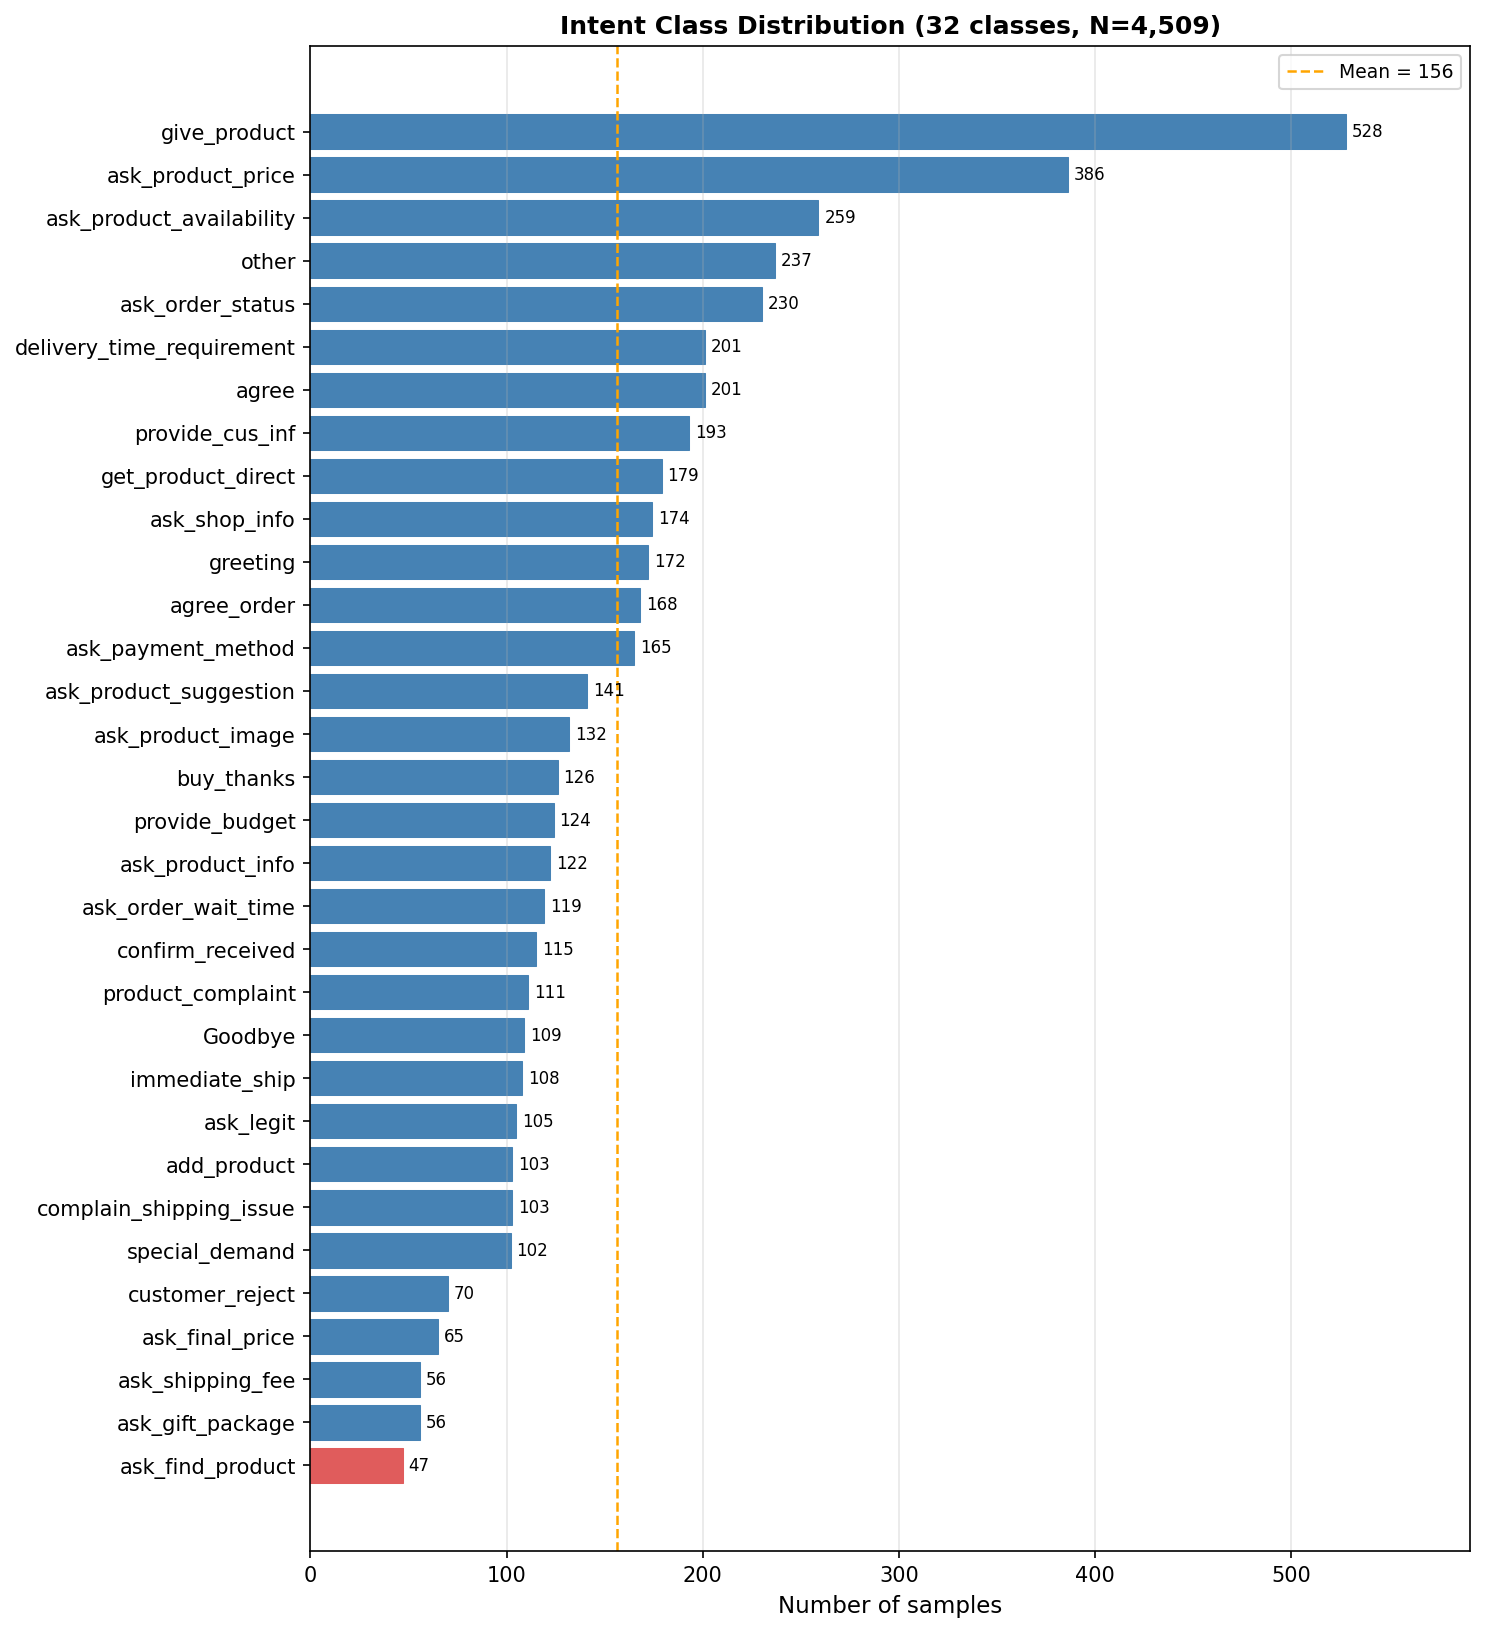
\includegraphics[width=0.95\linewidth]{intent_distribution.png}
\caption{Sample count distribution across 32 intent classes (N = 4,509 messages)}
\label{fig:intent_dist}
\end{figure}

\subsection{Message Length Distribution}

Most messages in the dataset are very short (1--10 words after segmentation),
reflecting the nature of real chat communication.
The longest messages typically occur when customers provide delivery addresses
or ask multiple questions in a single message.
This right-skewed distribution challenges the model:
with only 1--3 words, very little context is available to distinguish near-synonymous intent classes.

\subsection{Conversation Length Distribution}

Figure~\ref{fig:conv_length} shows the distribution of the number of messages
from the start of a conversation until the customer confirms an order or declines to purchase.

\begin{figure}[H]
\centering
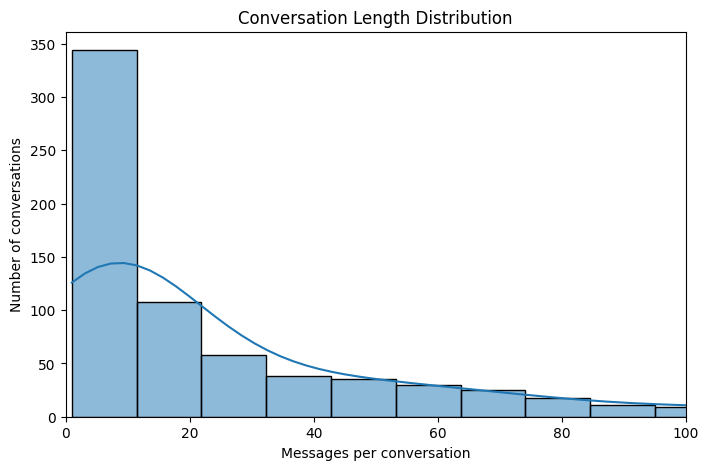
\includegraphics[width=0.85\linewidth]{conservation_length.png}
\caption{Distribution of conversation length (messages per conversation)}
\label{fig:conv_length}
\end{figure}

The distribution is strongly right-skewed:
the majority of conversations contain fewer than 10 messages,
the next largest group spans 10--20 messages,
and only a small number of conversations extend to 100 messages.
Longer conversations typically involve customers requesting additional product details,
comparing multiple options, or re-submitting invalid information.

\section{Data Preprocessing}

\subsection{Teen-Code Normalization}

The normalization step converts informal text to a more standard form
using a domain-specific dictionary, while protecting English tokens
(brand names) from incorrect substitution:

\begin{lstlisting}[language=Python, caption={Text normalization function}]
TEEN_CODE = {
    'k': 'khong', 'ko': 'khong', 'kh': 'khong',
    'dc': 'duoc', 'doc': 'duoc',
    'sop': 'shop',   'ck': 'chuyen khoan',
    'r': 'roi',      'nha': 'nhe',
    'sp': 'san pham', 'mn': 'moi nguoi',
}

def normalize(text: str) -> str:
    text = text.lower()
    text = re.sub(r'(.)\1{2,}', r'\1\1', text)   # collapse repeated chars
    out = []
    for tok in text.split():
        # Protect Latin tokens (brand names)
        if re.match(r'^[a-z0-9\-]+$', tok) and tok not in TEEN_CODE:
            out.append(tok)
        else:
            out.append(TEEN_CODE.get(tok, tok))
    return ' '.join(out)
\end{lstlisting}

Table~\ref{tab:teencode} lists the most common abbreviations in the dataset.

\begin{table}[H]
\centering
\caption{Teen-code normalization dictionary (excerpt)}
\label{tab:teencode}
\begin{tabular}{lll}
\toprule
\textbf{Teen-code} & \textbf{Standard form} & \textbf{Note} \\
\midrule
\texttt{k}, \texttt{ko}, \texttt{kh}, \texttt{khum} & kh\^ong (no) & Most common abbreviation \\
\texttt{dc}, \texttt{doc}  & du\textit{o}c (okay)   & \\
\texttt{vs}                & v\textit{o}i (with)    & \\
\texttt{sop}, \texttt{soc} & shop                   & Playful mispronunciation \\
\texttt{ck}                & chuyen khoan (bank transfer) & Business term \\
\texttt{r}, \texttt{rui}   & r\^oi (already)        & \\
\texttt{nha}, \texttt{nhen}& nhe (please/okay)      & \\
\texttt{sp}                & san pham (product)     & \\
\texttt{mn}                & moi nguoi (everyone)   & \\
\texttt{m}                 & minh (I/me)            & \\
\bottomrule
\end{tabular}
\end{table}

\subsection{Word Segmentation with underthesea}

After normalization, text is segmented using the underthesea library
to match the register of PhoBERT's pre-training data:

\begin{lstlisting}[language=Python, caption={Word segmentation with underthesea}]
from underthesea import word_tokenize

def segment(text: str) -> str:
    return word_tokenize(text, format='text')

# Examples:
# "ha noi"        -> "ha_noi"
# "chuyen khoan"  -> "chuyen_khoan"
# "san pham"      -> "san_pham"
\end{lstlisting}

\subsection{Dataset Splitting}

Since this is a multi-label classification problem, random splitting
may produce uneven label distributions across splits.
This thesis uses \textbf{Iterative Stratification} \cite{sechidis2011stratification}
from the \texttt{scikit-multilearn} library to ensure consistent label distributions:

\begin{center}
\textbf{80\% Train} / \textbf{10\% Validation} / \textbf{10\% Test}
\end{center}

The same split is used for all approaches to ensure a fair comparison.

\section{Data Augmentation}
\label{subsec:augmentation}

\subsection{Compositional Augmentation}

Rare intent class combinations (fewer than 5 co-occurring pairs) are augmented
by concatenating two single-label sentences to create synthetic multi-label samples:

\begin{lstlisting}[caption={Compositional augmentation example}]
# Original pair: ask_shipping_fee + ask_order_wait_time (only 4 samples)
"ship bao nhieu tien vay" + " voi " + "bao lau thi nhan duoc a"
=> labels: ["ask_shipping_fee", "ask_order_wait_time"]
\end{lstlisting}

4 target intent pairs $\times$ 40 samples/pair = \textbf{+160 synthetic samples}.

\subsection{Random Token Masking}

The full augmented training set is doubled by adding a masked copy
where 15\% of tokens are randomly replaced with \texttt{[MASK]}:

\begin{equation}
  \text{Expanded set} = 4{,}379 \text{ samples} \xrightarrow{\times 2} 8{,}758 \text{ samples}
\end{equation}

% ============================================================
%  CHAPTER 5 — INTENT CLASSIFICATION
% ============================================================
\chapter{Intent Classification}

\section{Problem Statement}

\textbf{Input:} An informal Vietnamese message
$x = (w_1, w_2, \ldots, w_n)$.

\textbf{Output:} Label set $\hat{Y} \subseteq \{c_1, c_2, \ldots, c_{32}\}$,
where each $c_i$ is a pre-defined intent class.

\textbf{Domain-specific challenges:}
\begin{itemize}
  \item Very short text (1--5 words) with insufficient discriminative context.
  \item Teen-code reduces the effectiveness of standard tokenizers.
  \item Severe class imbalance (10:1 ratio between the most and least frequent classes).
  \item Some class pairs have blurry semantic boundaries
        (e.g., \texttt{ask\_product\_info} vs. \texttt{ask\_product\_availability}).
\end{itemize}

\section{Approach 1 --- SVM + TF-IDF (Non-neural Baseline)}

\textbf{Rationale:} Establish a lower bound and verify whether deep learning
is truly necessary for this task.
SVM with TF-IDF handles code-switching naturally ---
\texttt{lego}, \texttt{ferrari}, and Vietnamese words are treated as
equally weighted features regardless of language.

\textbf{Configuration:}
\begin{itemize}
  \item TF-IDF: word unigrams + bigrams, max 50,000 features.
  \item Model: \texttt{OneVsRestClassifier(LinearSVC())},
        \texttt{class\_weight='balanced'}.
  \item No special preprocessing required.
\end{itemize}

\textbf{Limitation:} No lexical semantics captured ---
\texttt{k} and \texttt{kh\^ong} are treated as two different features
despite identical meaning; cannot handle out-of-vocabulary (OOV) terms.

\section{Approach 2 --- Fine-tune ViSoBERT}

\textbf{Hypothesis:} Pre-training on Vietnamese social media text
allows ViSoBERT to handle teen-code and code-switching
without any preprocessing.

\textbf{Architecture:}
\begin{equation}
  \text{ViSoBERT} \rightarrow h_{[\text{CLS}]} \rightarrow \text{Dropout}(0.3)
  \rightarrow \text{Linear}(768 \rightarrow 32) \rightarrow \sigma
\end{equation}

\textbf{Training configuration:} AdamW, lr $= 2 \times 10^{-5}$,
batch = 32, max 20 epochs, early stopping (patience = 5 on val Macro-F1).

\section{Approach 3 --- Fine-tune PhoBERT + Normalization + Word Segmentation}
\label{sec:approach3}

\textbf{Hypothesis:} Explicit text normalization allows PhoBERT to leverage
its pre-training knowledge from formal text,
compensating for the train-inference register mismatch.

\subsection{Model Architecture}
\label{subsec:approach3_arch}

\begin{table}[H]
\centering
\caption{Model architecture parameters for Approach 3}
\label{tab:arch_params}
\begin{tabular}{ll}
\toprule
\textbf{Component} & \textbf{Detail} \\
\midrule
Base model              & \texttt{vinai/phobert-base} (BERT-base, BPE vocab 64K) \\
Total parameters        & 135M \\
Trainable parameters    & $\approx$ 40M (encoder layers 5--12 + head) \\
Hidden size             & 768-dim \\
Encoder layers          & 12 (layers 1--4 frozen, layers 5--12 trainable) \\
Classification head     & Linear($768 \rightarrow 32$) + Sigmoid \\
Dropout                 & $p = 0.3$ on $h_{[\texttt{CLS}]}$ \\
Max sequence length     & 128 tokens \\
\bottomrule
\end{tabular}
\end{table}

The overall architecture consists of four cascaded stages:

\begin{enumerate}
  \item \textbf{Text preprocessing:}
        Lowercase $\rightarrow$ teen-code normalization (dictionary) $\rightarrow$
        protect Latin tokens (brand names) $\rightarrow$
        \texttt{underthesea.word\_tokenize()}.
  \item \textbf{PhoBERT Tokenizer:} BPE, vocab 64K, max\_len = 128 tokens
        (truncate + pad). Output: \texttt{[CLS]} $w_1 \cdots w_n$ \texttt{[SEP]}.
  \item \textbf{PhoBERT-base Encoder:} 12 transformer layers, 768-dim hidden;
        layers 1--4 frozen; output $h_{[\texttt{CLS}]} \in \mathbb{R}^{768}$.
  \item \textbf{Classification Head:}
        $\text{Dropout}(0.3) \rightarrow \text{Linear}(768 \rightarrow 32)
        \rightarrow \sigma$.
\end{enumerate}

Final classification:

\begin{equation}
  \hat{y}_i = \mathbf{1}\!\left[\sigma\!\left(W h_{[\texttt{CLS}]} + b\right)_i \geq t_i\right],
  \quad i = 1, \ldots, 32
\end{equation}

where $t_i$ is a per-class threshold optimized on the validation set.

\subsection{Training Workflow}
\label{subsec:approach3_workflow}

\begin{table}[H]
\centering
\caption{Training workflow for Approach 3}
\label{tab:training_workflow}
\begin{tabularx}{\linewidth}{clX}
\toprule
\textbf{Step} & \textbf{Name} & \textbf{Description} \\
\midrule
1 & Data preparation
  & Load train set (8,758 samples after augmentation),
    val (10\%), test (10\%) via Iterative Stratification. \\
2 & Preprocessing
  & Each sample passes through \texttt{normalize()} $\rightarrow$
    \texttt{word\_tokenize()} $\rightarrow$ PhoBERT tokenizer
    (truncate/pad to 128 tokens). \\
3 & Model initialization
  & Load \texttt{vinai/phobert-base};
    freeze embedding + encoder layers 1--4;
    attach classification head Linear($768 \rightarrow 32$). \\
4 & Compute pos\_weight
  & $w_i = (N - n_i) / n_i$ for each class $i$,
    passed to \texttt{BCEWithLogitsLoss(pos\_weight=...)}. \\
5 & Training
  & AdamW (lr $= 2\!\times\!10^{-5}$, weight\_decay $= 0.05$),
    linear warmup 10\% steps $\rightarrow$ linear decay,
    gradient clipping max\_norm $= 1.0$,
    batch $= 32$, max 30 epochs. \\
6 & Early stopping
  & Monitor val Macro-F1 after each epoch;
    stop if no improvement for 5 consecutive epochs;
    save best checkpoint. \\
7 & Threshold tuning
  & Grid search $t_i \in [0.3,\,0.7]$ (step 0.01) on val set
    to maximize Macro-F1 per class across all 32 classes;
    save vector $\mathbf{t} = (t_1,\ldots,t_{32})$. \\
8 & Evaluation
  & Apply $\mathbf{t}$ on test set;
    compute Macro-F1, Micro-F1, Hamming Loss, Subset Accuracy. \\
\bottomrule
\end{tabularx}
\end{table}

\subsection{Loss Function and Optimizer}
\label{subsec:approach3_loss}

The Binary Cross-Entropy loss with pos\_weight handles class imbalance:

\begin{equation}
  \mathcal{L} = -\frac{1}{C}\sum_{i=1}^{C}
  \Bigl[ w_i \cdot y_i \log\sigma(z_i)
       + (1 - y_i)\log(1-\sigma(z_i)) \Bigr],
  \quad w_i = \frac{N - n_i}{n_i}
\label{eq:bce_loss}
\end{equation}

where $N$ is the total number of samples and $n_i$ is the number of positive samples
for class $i$. This formula automatically increases gradient weight for rare classes.

The learning rate schedule uses a linear warmup over the first 10\% of training steps,
followed by linear decay to zero:

\begin{equation}
  \text{lr}(s) =
  \begin{cases}
    \text{lr}_0 \cdot \dfrac{s}{s_\mathrm{warm}} & s < s_\mathrm{warm} \\[6pt]
    \text{lr}_0 \cdot \dfrac{S - s}{S - s_\mathrm{warm}} & s \geq s_\mathrm{warm}
  \end{cases}
\label{eq:lr_schedule}
\end{equation}

\subsection{Inference Pipeline}
\label{subsec:approach3_inference}

At deployment, the inference pipeline is condensed to:

\begin{center}
$\text{raw}$
$\xrightarrow{\texttt{normalize()}}$
$\text{segmented}$
$\xrightarrow{\text{tokenizer}}$
$\text{token IDs}$
$\xrightarrow{\text{PhoBERT}}$
$h_{[\texttt{CLS}]}$
$\xrightarrow{\text{head}+\sigma}$
$\mathbf{p}$
$\xrightarrow{t_i}$
$\hat{Y}$
\end{center}

The entire inference pass runs inside a \texttt{torch.no\_grad()} context,
with average latency $\approx 20$--$50$\,ms on CPU.

\subsection{Additional Techniques in the Final Model}
\label{subsec:approach3_tricks}

\begin{itemize}
  \item \textbf{Layer freezing:} Freeze the embedding layer and the first 4 of 12 encoder layers.
        Reason: without freezing, train loss collapsed to $\approx 0.003$
        while val F1 plateaued --- a typical sign of overfitting when fine-tuning BERT
        on a small dataset. The lower layers already encode Vietnamese syntax
        from pre-training and do not need further updating.
  \item \textbf{Weight decay 0.05:} Increased from the default 0.01
        to add regularization for the trainable layers.
  \item \textbf{Data augmentation:} 4,379 $\rightarrow$ 8,758 samples
        (compositional augmentation + 15\% random masking, see \S\ref{subsec:augmentation}).
  \item \textbf{Per-class threshold tuning:} Grid search for $t_i$
        maximizing Macro-F1 on the val set for each of the 32 classes,
        instead of using a fixed threshold of 0.5 for all classes.
\end{itemize}

\section{Approach 4 --- Fine-tune XLM-RoBERTa}

\textbf{Hypothesis:} Multilingual pre-training creates strong representations
for both Vietnamese and English brand names in the same embedding space,
directly addressing the code-switching challenge.

\textbf{Characteristics:} 278M parameters (twice the size of PhoBERT-base at 135M);
SentencePiece tokenizer handles mixed-language input without word segmentation.

\section{Evaluation and Comparison}

\subsection{Overall Comparison of 4 Approaches}

\begin{table}[H]
\centering
\caption{Comparison of 4 intent classification approaches on the test set}
\label{tab:intent_compare}
\begin{tabular}{lcccc}
\toprule
\textbf{Approach} & \textbf{Macro-F1} & \textbf{Micro-F1} & \textbf{Hamming} & \textbf{Subset Acc} \\
\midrule
SVM + TF-IDF (C=10)   & 0.8695 & 0.8727 & 0.0090 & 0.7600 \\
ViSoBERT              & \textbf{0.9248} & \textbf{0.9254} & \textbf{0.0052} & \textbf{0.8711} \\
PhoBERT + Norm + Seg  & 0.9022 & 0.9073 & 0.0065 & 0.8533 \\
XLM-RoBERTa           & \placeholder{results pending} & --- & --- & --- \\
\bottomrule
\end{tabular}
\end{table}

\subsection{Per-class Evaluation of the Deployed Model (Approach 3)}

Table~\ref{tab:perclass_intent} reports the F1 score per class
for the PhoBERT + Norm + Seg model on the test set.

\begin{longtable}{lc}
\caption{Per-class F1 for Approach 3 (PhoBERT + Norm + Seg) on the test set}
\label{tab:perclass_intent} \\
\toprule
\textbf{Intent} & \textbf{F1} \\
\midrule
\endfirsthead
\multicolumn{2}{c}{\textit{(continued from Table~\ref{tab:perclass_intent})}} \\
\toprule
\textbf{Intent} & \textbf{F1} \\
\midrule
\endhead
\bottomrule
\endlastfoot
\texttt{Goodbye}                    & \textbf{1.0000} \\
\texttt{add\_product}               & \textbf{1.0000} \\
\texttt{ask\_payment\_method}       & \textbf{1.0000} \\
\texttt{ask\_product\_info}         & \textbf{1.0000} \\
\texttt{ask\_shop\_info}            & \textbf{1.0000} \\
\texttt{confirm\_received}          & \textbf{1.0000} \\
\texttt{customer\_reject}           & \textbf{1.0000} \\
\texttt{get\_product\_direct}       & \textbf{1.0000} \\
\texttt{ask\_order\_status}         & 0.9778 \\
\texttt{ask\_product\_price}        & 0.9867 \\
\texttt{delivery\_time\_requirement}& 0.9744 \\
\texttt{provide\_budget}            & 0.9630 \\
\texttt{provide\_cus\_inf}          & 0.9500 \\
\texttt{greeting}                   & 0.9412 \\
\texttt{ask\_order\_wait\_time}     & 0.9167 \\
\texttt{agree\_order}               & 0.9143 \\
\texttt{ask\_gift\_package}         & 0.9231 \\
\texttt{ask\_product\_image}        & 0.9231 \\
\texttt{buy\_thanks}                & 0.9231 \\
\texttt{complain\_shipping\_issue}  & 0.9091 \\
\texttt{product\_complaint}         & 0.9091 \\
\texttt{ask\_product\_availability} & 0.8889 \\
\texttt{ask\_product\_suggestion}   & 0.8750 \\
\texttt{immediate\_ship}            & 0.8696 \\
\texttt{agree}                      & 0.8649 \\
\texttt{special\_demand}            & 0.8421 \\
\texttt{ask\_legit}                 & 0.8235 \\
\texttt{ask\_shipping\_fee}         & 0.8000 \\
\texttt{other}                      & 0.7917 \\
\texttt{ask\_final\_price}          & 0.7692 \\
\texttt{give\_product}              & 0.7339 \\
\texttt{ask\_find\_product}         & 0.4000 \\
\end{longtable}

Figure~\ref{fig:perclass_f1} visualizes the results above,
with red bars marking classes below the Macro-F1 mean.

\begin{figure}[H]
\centering
\begin{subfigure}[b]{0.49\linewidth}
  \includegraphics[width=\linewidth]{approach3_results/results/per_class_f1.png}
  \caption{Approach 3 --- PhoBERT + Norm (Macro-F1 = 0.902)}
\end{subfigure}
\hfill
\begin{subfigure}[b]{0.49\linewidth}
  \includegraphics[width=\linewidth]{approach2/results/per_class_f1.png}
  \caption{Approach 2 --- ViSoBERT (Macro-F1 = 0.925)}
\end{subfigure}
\caption{Per-class F1 on the test set: PhoBERT (left) vs. ViSoBERT (right).
         Dashed line = overall Macro-F1; red bars = classes below average.}
\label{fig:perclass_f1}
\end{figure}

\textbf{Observations:}
\begin{itemize}
  \item 8 classes achieve F1 = 1.00: these intents have unambiguous semantics
        with little overlap with other classes.
  \item \texttt{ask\_find\_product} achieves F1 = 0.40 because the test set
        contains only 4 samples --- too few for reliable evaluation.
  \item Classes with intermediate F1 (0.73--0.89) typically have
        blurry semantic boundaries with neighboring classes.
\end{itemize}

\subsection{Learning Curve Analysis}

Before applying layer freezing, train loss collapsed to $\approx 0.003$
while val Macro-F1 plateaued and failed to improve after epoch 8 ---
a typical sign of overfitting.
After freezing the first 4 encoder layers, val Macro-F1 improved steadily
and converged at epoch 21 (val Macro-F1 = 0.8769).
Figure~\ref{fig:approach3_curves} illustrates the training process.

\begin{figure}[H]
\centering
\begin{subfigure}[b]{0.49\linewidth}
  \includegraphics[width=\linewidth]{approach3_results/results/training_curves.png}
  \caption{Approach 3 --- PhoBERT + Norm (best epoch: 21)}
  \label{fig:curve_approach3}
\end{subfigure}
\hfill
\begin{subfigure}[b]{0.49\linewidth}
  \includegraphics[width=\linewidth]{approach2/results/training_curves.png}
  \caption{Approach 2 --- ViSoBERT (best epoch: 10)}
  \label{fig:curve_approach2}
\end{subfigure}
\caption{Training curves: Train Loss (orange) and Val Macro-F1 (blue dashed, right axis)}
\label{fig:approach3_curves}
\end{figure}

ViSoBERT converges faster (epoch 10) due to its social media pre-training.
PhoBERT requires more epochs (21), but with normalization + word segmentation,
the model gradually exploits its pre-training knowledge from formal text.

\subsection{Ablation Study}

\begin{table}[H]
\centering
\caption{Ablation study --- contribution of each technique in Approach 3}
\label{tab:ablation}
\begin{tabular}{lcc}
\toprule
\textbf{Configuration} & \textbf{Val Macro-F1} & \textbf{Test Macro-F1} \\
\midrule
PhoBERT baseline (no preprocessing)  & \placeholder{} & \placeholder{} \\
+ Teen-code normalization             & \placeholder{} & \placeholder{} \\
+ Word segmentation (underthesea)     & \placeholder{} & \placeholder{} \\
+ Layer freezing                      & \placeholder{} & \placeholder{} \\
+ Augmentation (comp. + masking)      & \placeholder{} & \textbf{0.9022} \\
\bottomrule
\end{tabular}
\end{table}

\subsection{Error Analysis}

Analysis of the most common misclassification patterns:

\begin{itemize}
  \item \textbf{Error 1 --- Very short input:}
        ``\textit{ok}'' is misclassified between \texttt{agree\_order}
        and \texttt{Goodbye} due to lack of context.
  \item \textbf{Error 2 --- Out-of-dictionary teen-code:}
        Creative abbreviations absent from the normalization dictionary
        result in tokens that are not correctly recognized.
  \item \textbf{Error 3 --- Near-synonymous intents:}
        \texttt{ask\_product\_info} and \texttt{ask\_product\_availability}
        both take the form of product questions and are easily confused with short inputs.
  \item \textbf{Error 4 --- Rare classes:}
        Classes with fewer than 50 training samples still exhibit unstable F1.
\end{itemize}

\subsection{Chapter Summary}

Approach 3 (PhoBERT + normalization + word segmentation) achieves Macro-F1 = 0.9022,
outperforming the other non-neural approach.
This result confirms the research hypothesis: explicit text normalization
combined with word segmentation can compensate for PhoBERT's formal-text pre-training
when applied to informal chat data.

% ============================================================
%  CHAPTER 6 — NER
% ============================================================
\chapter{Named Entity Recognition (NER)}

\section{Problem Statement}

\textbf{Input:} Raw Vietnamese message (not normalized, to preserve
brand names and phone numbers).

\textbf{Output:} List of entities $(span, label)$ with 13 entity types:

\begin{table}[H]
\centering
\caption{13 entity types in the system}
\label{tab:entities}
\begin{tabular}{lll}
\toprule
\textbf{Group} & \textbf{Entity} & \textbf{Example} \\
\midrule
\multirow{4}{*}{Customer}
  & \texttt{NAME}    & Nguyen Thanh \\
  & \texttt{PHONE}   & 0868928485 \\
  & \texttt{ADDRESS} & 30 ngo 20 Cat Linh \\
  & \texttt{CITY}    & Ha Noi \\
\midrule
\multirow{2}{*}{Budget}
  & \texttt{MAX\_BUDGET} & 900k \\
  & \texttt{MIN\_BUDGET} & around 500 \\
\midrule
\multirow{4}{*}{Product}
  & \texttt{PRODUCT\_NAME}  & Porsche 911 \\
  & \texttt{TYPE}           & car \\
  & \texttt{COMPLEXITY}     & hard \\
  & \texttt{PRODUCT\_COLOR} & red \\
\midrule
\multirow{3}{*}{Order}
  & \texttt{QUANTITY}   & 2 sets \\
  & \texttt{SHIP\_DATE} & tomorrow \\
  & \texttt{SHIP\_TIME} & morning \\
\bottomrule
\end{tabular}
\end{table}

\section{Method 1 --- PhoBERT Fine-tuned for NER}

PhoBERT uses a BPE tokenizer derived from formal Vietnamese text.
English brand names such as ``Porsche'' and ``Ferrari''
are split into low-semantics subwords (\texttt{\_Por}, \texttt{sche}),
weakening \texttt{PRODUCT\_NAME} recognition.

\textbf{Aggregation strategy:} Each word's label is determined by its first subword
(first-subword aggregation); subsequent subwords of the same word are discarded
when consolidating predictions.

\textbf{Result:} Micro-F1 $\approx 0.61$.

\section{Method 2 --- ViSoBERT Fine-tuned for NER}

ViSoBERT, pre-trained on Vietnamese social media text,
has a richer vocabulary for e-commerce terms and English brand names
compared to PhoBERT.

\textbf{Training configuration:} Same as Approach 2 in Chapter 5
(AdamW, lr $= 2 \times 10^{-5}$, batch = 16, max 20 epochs,
early stopping patience = 5 on val Micro-F1).

\textbf{Result:} Micro-F1 $\approx 0.70$.

\section{Evaluation and Comparison}

\subsection{Overall Comparison}

\begin{table}[H]
\centering
\caption{Comparison of PhoBERT and ViSoBERT for NER}
\label{tab:ner_compare}
\begin{tabular}{lccc}
\toprule
\textbf{Model} & \textbf{Precision} & \textbf{Recall} & \textbf{Micro-F1} \\
\midrule
PhoBERT NER              & 0.5525 & 0.7393 & 0.6324 \\
\textbf{ViSoBERT NER v2} & \textbf{0.6623} & \textbf{0.7937} & \textbf{0.7220} \\
\bottomrule
\end{tabular}
\end{table}

Figure~\ref{fig:ner_curves} shows the training curves for both models.
ViSoBERT converges at epoch 45, while PhoBERT requires up to epoch 80 ---
reflecting ViSoBERT's better fit with informal chat data.

\begin{figure}[H]
\centering
\begin{subfigure}[b]{0.49\linewidth}
  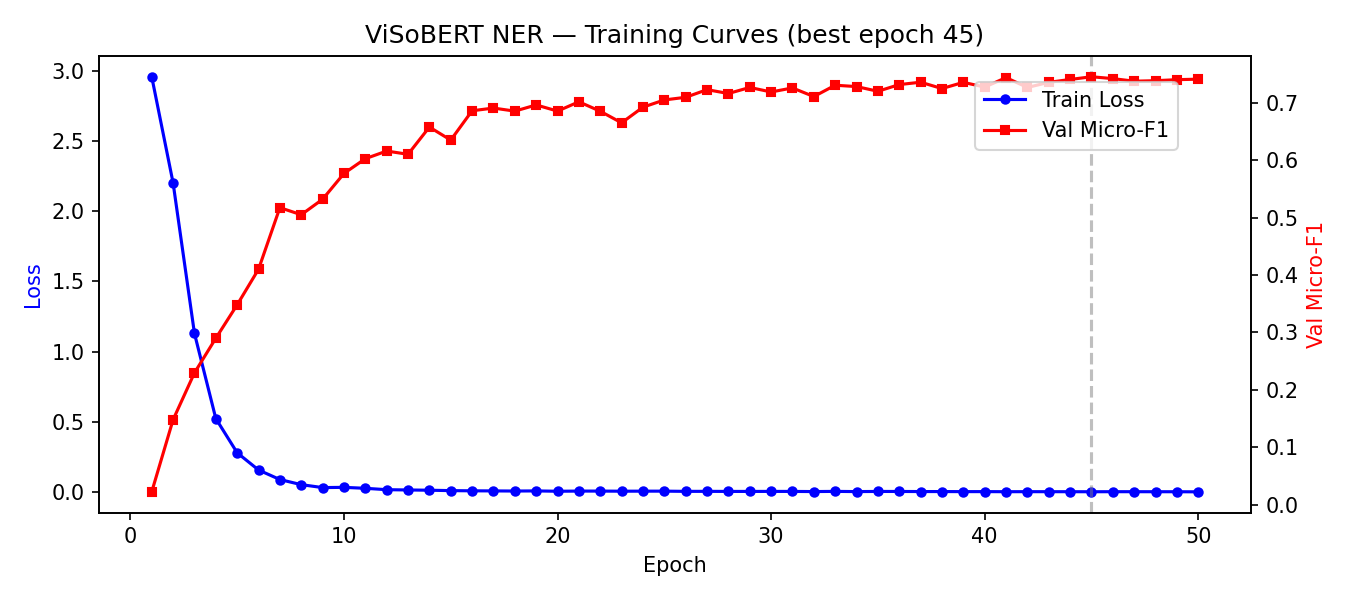
\includegraphics[width=\linewidth]{ner/results/ner_training_curves.png}
  \caption{ViSoBERT NER (best epoch: 45, val Micro-F1 $\approx$ 0.73)}
\end{subfigure}
\hfill
\begin{subfigure}[b]{0.49\linewidth}
  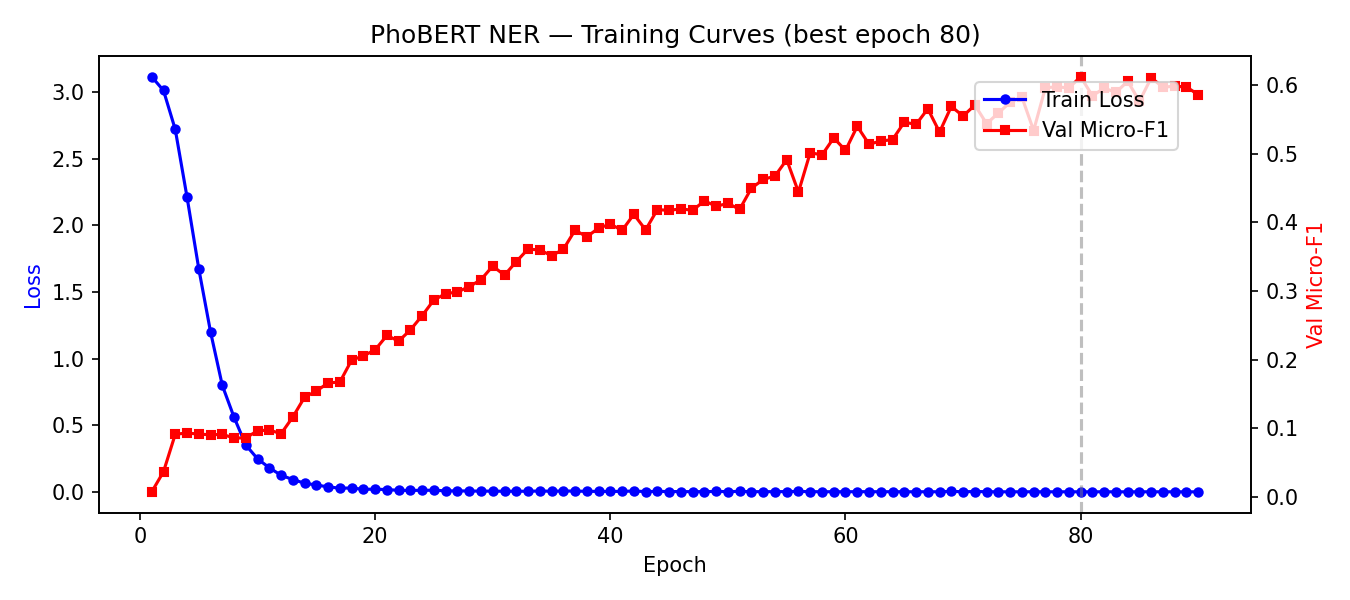
\includegraphics[width=\linewidth]{ner/results/ner_phobert_training_curves.png}
  \caption{PhoBERT NER (best epoch: 80, val Micro-F1 $\approx$ 0.60)}
\end{subfigure}
\caption{NER training curves: Train Loss (blue) and Val Micro-F1 (red)}
\label{fig:ner_curves}
\end{figure}

\subsection{Per-entity-type Comparison}

\begin{table}[H]
\centering
\caption{Per-entity-type F1: PhoBERT vs. ViSoBERT}
\label{tab:ner_pertype}
\begin{tabular}{lccl}
\toprule
\textbf{Entity} & \textbf{PhoBERT F1} & \textbf{ViSoBERT F1} & \textbf{Note} \\
\midrule
\texttt{NAME}          & 0.9412 & 0.9200 & Often sentence-initial \\
\texttt{PHONE}         & 0.9091 & \textbf{1.0000} & Digit pattern easy to detect \\
\texttt{ADDRESS}       & 0.3729 & 0.8475 & Most complex, diverse syntax \\
\texttt{CITY}          & 0.5000 & 0.7273 & \\
\texttt{PRODUCT\_NAME} & 0.6180 & 0.6791 & ViSoBERT clearly better \\
\texttt{MAX\_BUDGET}   & 0.8800 & 0.9474 & Pattern ``Nk'', ``N million'' \\
\texttt{MIN\_BUDGET}   & 0.9286 & 0.9143 & \\
\texttt{QUANTITY}      & 0.9000 & 0.9000 & \\
\texttt{SHIP\_DATE}    & 0.4444 & 0.6000 & ``tomorrow'', ``Tuesday'' \\
\texttt{SHIP\_TIME}    & 0.6923 & 0.7692 & \\
\texttt{TYPE}          & 0.5556 & 0.4828 & \\
\texttt{COMPLEXITY}    & 0.5149 & 0.4667 & Hardest entity for both models \\
\texttt{PRODUCT\_COLOR}& 0.5926 & 0.6154 & \\
\bottomrule
\end{tabular}
\end{table}

\begin{figure}[H]
\centering
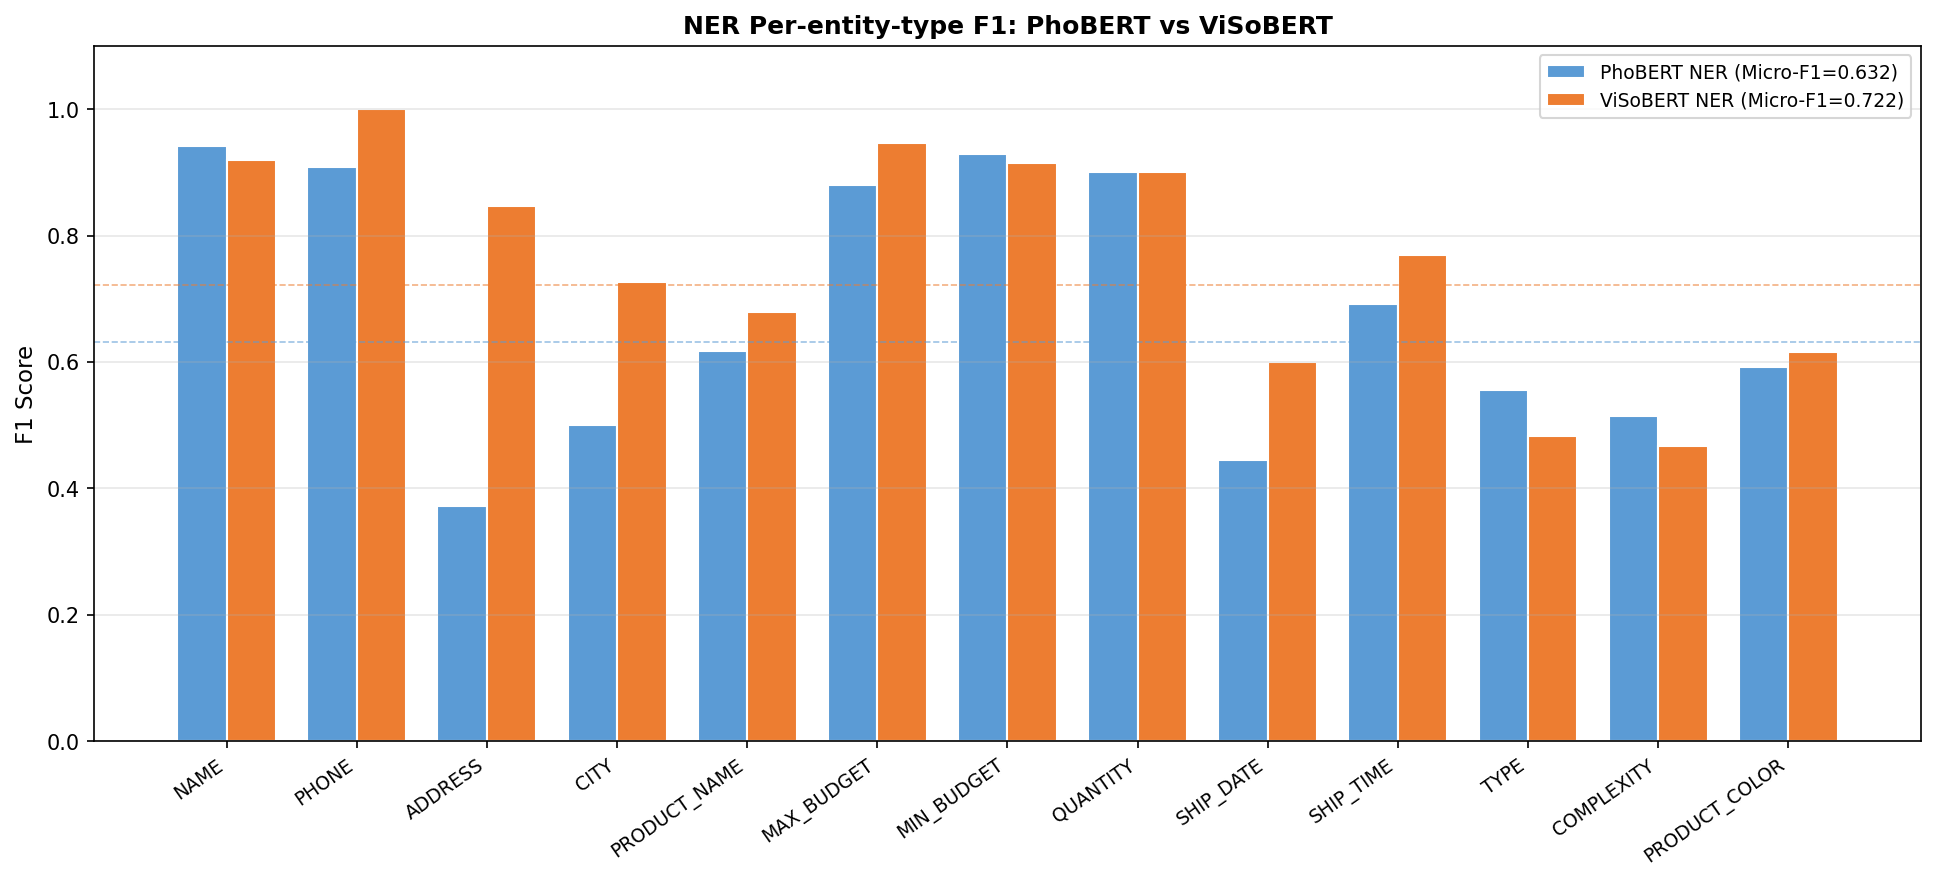
\includegraphics[width=0.95\linewidth]{ner_comparison.png}
\caption{Per-entity-type F1 comparison between PhoBERT and ViSoBERT.
         Dashed lines = overall Micro-F1 for each model.}
\label{fig:ner_comparison}
\end{figure}

From Figure~\ref{fig:ner_comparison}, ViSoBERT outperforms PhoBERT on most entity types,
especially \texttt{ADDRESS} (+0.47), \texttt{CITY} (+0.23), and \texttt{SHIP\_DATE} (+0.16).
PhoBERT is only marginally better on \texttt{NAME} (+0.02) and \texttt{MIN\_BUDGET} (+0.01).
\texttt{COMPLEXITY} and \texttt{TYPE} are the most challenging entities for both models,
reflecting their abstract, context-dependent nature.

\subsection{NER Error Analysis}

\begin{itemize}
  \item \textbf{Boundary errors:} The model sometimes starts or ends a span
        one token off. Most common with \texttt{ADDRESS},
        as Vietnamese addresses have no fixed syntactic structure.
  \item \textbf{Type confusion:} \texttt{PRODUCT\_NAME} is confused with \texttt{TYPE}
        when the customer refers only to a general product category
        (``toy car'', ``house set'') without specifying a product name.
  \item \textbf{Low-resource entities:} \texttt{COMPLEXITY} and
        \texttt{PRODUCT\_COLOR} have low F1 scores due to limited training examples.
\end{itemize}

\subsection{Data--Performance Correlation}

Entities with the highest F1 scores are those with clear, repetitive patterns
(\texttt{PHONE}, \texttt{QUANTITY}). Entities with the lowest F1 correspond to
small training sets and complex semantic characteristics (\texttt{ADDRESS}).

\section{Post-processing: Product Matching}

After NER returns a \texttt{PRODUCT\_NAME} span, the \texttt{product\_matcher.py} module
performs fuzzy matching against the 11,362-item product catalog:

\begin{enumerate}
  \item \textbf{Fuzzy match:} \texttt{rapidfuzz.fuzz.token\_set\_ratio}
        compares the span against all product names; the top-3 highest-scoring candidates are retained.
  \item \textbf{Semantic fallback:} If the fuzzy score is low,
        cosine similarity on embeddings is used to find the nearest semantic match.
\end{enumerate}

The resulting top-3 candidate list is presented to the customer for confirmation
before adding to the order.

\section{Chapter Summary}

ViSoBERT outperforms PhoBERT on NER (Micro-F1 $\approx 0.72$ vs. $0.63$),
especially for \texttt{PRODUCT\_NAME} containing English brand names.
This contrasts with intent classification results, where PhoBERT + normalization
outperforms ViSoBERT, indicating that the two tasks have different requirements:
NER requires recognizing named entities at the token level,
while intent classification requires understanding sentence-level semantics.

% ============================================================
%  CHAPTER 7 — CHATBOT SYSTEM ARCHITECTURE
% ============================================================
\chapter{Chatbot System Architecture}

\section{Architecture Overview}

The system is built on FastAPI and supports two processing modes
running in parallel on the same endpoint:

\begin{lstlisting}[caption={Main API endpoint}]
POST /chat
{
  "session_id": "abc",
  "message": "I want the Porsche please",
  "mode": "hybrid" | "llm_full",
  "reply_to_msg_id": "m12"   // Messenger-style reply
}
\end{lstlisting}

Each conversation turn is logged to a JSONL file
(\texttt{logs/chat\_YYYYMMDD.jsonl}) for later analysis.
Session state is stored in-memory by \texttt{session\_id},
and completed orders are persisted to SQLite.

\section{Hybrid Pipeline (NLU + Rule-based)}

\subsection{Processing Flow}

\begin{center}
\texttt{message} $\rightarrow$ \texttt{nlu.py} $\rightarrow$
\texttt{pipeline.py} $\rightarrow$ \texttt{reply.py} $\rightarrow$ \texttt{response}
\end{center}

\begin{enumerate}
  \item \textbf{NLU:} PhoBERT classifies 32 intents (multi-label) +
        ViSoBERT extracts 13 entity types.
  \item \textbf{Pipeline:} 14 rule-based branches run sequentially by priority;
        the first branch that sets an \texttt{action} wins.
  \item \textbf{Reply:} Template generates a response based on \texttt{action}
        and the current slot state.
\end{enumerate}

\subsection{14-Branch Pipeline}

\begin{table}[H]
\centering
\caption{14 pipeline branches in priority order}
\label{tab:pipeline}
\begin{tabularx}{\linewidth}{llX}
\toprule
\textbf{Branch} & \textbf{Condition} & \textbf{Action} \\
\midrule
A.0      & \texttt{stage=done} + new greeting      & Reset cart, keep customer info \\
A.0-done & \texttt{stage=done} (other intent)       & Lock pipeline, prompt to send bill \\
A.1      & \texttt{pending\_availability} + affirm  & Auto-add product to cart \\
A.3--A.5 & pending\_finalize/cancel/mid-flow cancel & Request confirmation before action \\
B        & await\_payment/confirm/info              & Continue order flow \\
B2       & Information inquiry intent               & Answer, do not add to cart \\
C        & \texttt{customer\_reject} + pending      & Reject proposal \\
D        & Select number from proposal              & Confirm (propose) or ask more (suggest) \\
E        & Has \texttt{PRODUCT\_NAME}/type/color    & Propose top-3 from matcher \\
F        & \texttt{agree\_order} / affirm + cart    & Enter order finalization flow \\
G        & \texttt{ask\_payment}/\texttt{ask\_suggestion} & Ask payment / suggest \\
H        & Q\&A intent (price, shipping, gift...)   & Respond directly \\
I        & \texttt{provide\_cus\_inf} + complete info & Proactively suggest order placement \\
J        & 5 consecutive unhandled turns            & Escalate $\rightarrow$ staff \\
\bottomrule
\end{tabularx}
\end{table}

\subsection{State Machine}

The order stage (\texttt{order\_stage}) is managed by a state machine:

\begin{equation}
  \texttt{None} \rightarrow \texttt{await\_info} \rightarrow
  \texttt{await\_confirm} \rightarrow \texttt{await\_payment} \rightarrow
  \texttt{done}
\end{equation}

\section{RAG System}

\subsection{Index Construction}

All 11,362 products are embedded using Gemini Embedding
(\texttt{models/gemini-embedding-2}) on first launch,
with results cached to an \texttt{.npy} file to avoid recomputation.
This process takes approximately 2--5 minutes and runs in a background thread
(lazy initialization) to avoid blocking the server.

\subsection{Hybrid Retrieval}

Instead of pure cosine search, the system uses hybrid retrieval
to ensure specific brand names always appear in the LLM context:

\begin{enumerate}
  \item \textbf{Keyword match:} Extract Latin tokens $\geq$ 4 characters
        from the query (\texttt{porsche}, \texttt{technic}, \texttt{ferrari}).
        Find all products containing these tokens in their names.
  \item \textbf{Cosine fill:} Fill remaining top-$k$ slots with products
        having the highest cosine similarity to the query embedding.
  \item \textbf{Merge:} Keyword match results are prioritized at the top
        (re-ranked by cosine score within the keyword group),
        followed by cosine results.
\end{enumerate}

\section{Full-LLM Baseline (Gemini 2.5 Flash Lite)}

\subsection{Pipeline}

\begin{center}
\texttt{message} $\rightarrow$ RAG (top-$k$ products) $\rightarrow$
build prompt $\rightarrow$ Gemini generate $\rightarrow$ reply + log
\end{center}

\textbf{Prompt structure:}
\begin{itemize}
  \item System instruction: LEGO sales advisor role and business rules.
  \item Product context: names, prices, and categories of retrieved products (from RAG).
  \item Conversation history: last 10 turns.
  \item User message.
\end{itemize}

\subsection{Logging}

Each LLM turn additionally logs:
\texttt{llm\_tokens\_in}, \texttt{llm\_tokens\_out},
\texttt{rag\_products}, \texttt{latency\_ms}.

\section{Frontend and Metrics Dashboard}

The frontend is built with plain HTML/CSS/JS, simulating a Messenger-style interface
to support the ``reply-to'' feature (replying to a specific message),
which is essential for the multi-turn product confirmation flow.

The \texttt{/metrics} page displays a live comparison of both modes:
average latency, total token consumption, estimated cost (VND),
and the list of orders in SQLite.

% ============================================================
\section{Use Cases}
\label{sec:usecases}

Figure~\ref{fig:usecases} presents the overall Use Case Diagram of the system,
with three main actors: \textbf{Customer}, \textbf{Staff}, and \textbf{Manager}.

\begin{figure}[H]
\centering
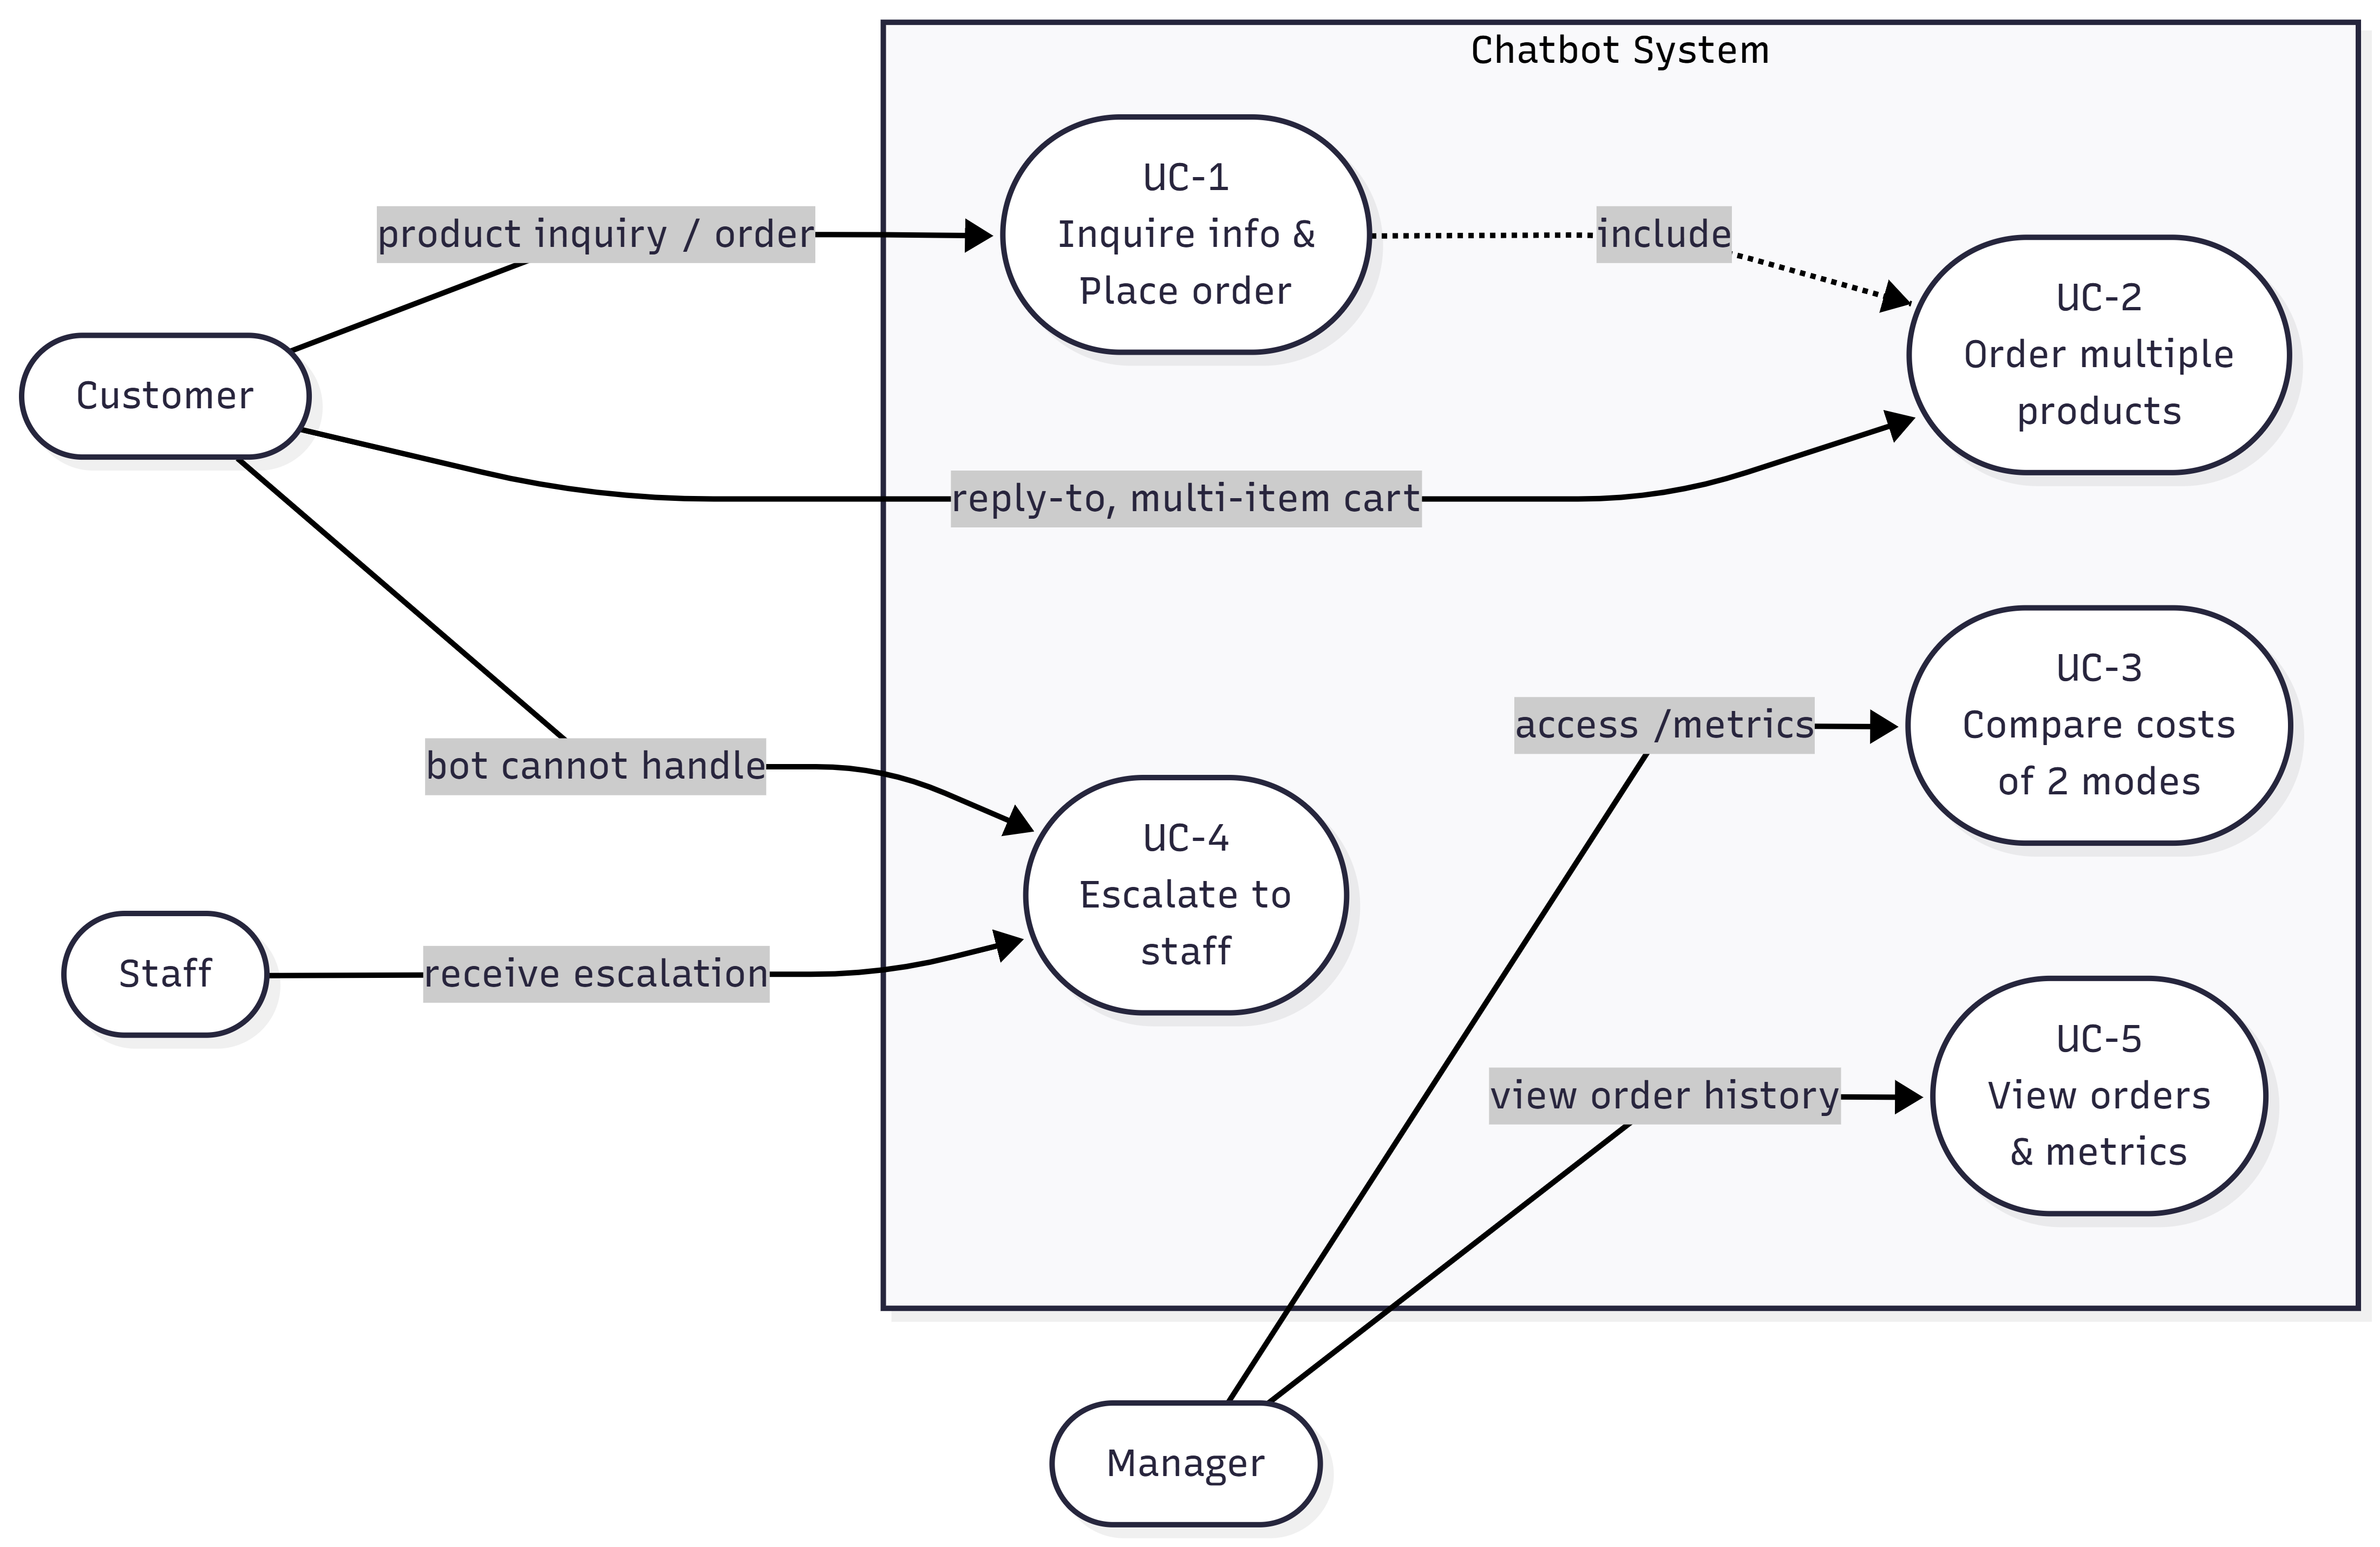
\includegraphics[width=0.92\linewidth]{Usecase.png}
\caption{Use Case Diagram --- LEGO Chatbot System}
\label{fig:usecases}
\end{figure}

\begin{table}[H]
\centering
\caption{Description of main use cases}
\label{tab:usecases}
\begin{tabularx}{\linewidth}{llX}
\toprule
\textbf{ID} & \textbf{Name} & \textbf{Brief description} \\
\midrule
UC-1 & Inquire \& place order
  & Customer inquires $\rightarrow$ bot recommends top-3
    $\rightarrow$ customer confirms $\rightarrow$ provides info
    $\rightarrow$ confirms payment $\rightarrow$ order saved. \\
UC-2 & Multi-product order
  & Customer uses reply-to to select multiple products;
    cart accumulates before checkout. \\
UC-3 & Compare cost of 2 modes
  & Manager views \texttt{/metrics}: latency, tokens,
    estimated cost between hybrid and full-LLM modes. \\
UC-4 & Escalate to staff
  & Bot fails to handle 5 consecutive turns (branch J)
    $\rightarrow$ transfers to staff with full context. \\
UC-5 & View orders \& metrics
  & Manager views order history in SQLite and JSONL logs. \\
\bottomrule
\end{tabularx}
\end{table}

\subsection{UC-1 Detail: Inquire and Place Order}

\textbf{Precondition:} Customer opens chat interface. \\
\textbf{Main flow:}
\begin{enumerate}
  \item Customer types: ``Do you still have the Ferrari?''
  \item Bot classifies intent (\texttt{ask\_product\_availability}),
        NER extracts \texttt{PRODUCT\_NAME = ``Ferrari''};
        matcher returns top-3 from the 11,362-item catalog.
  \item Customer selects: ``number 1''; bot confirms and requests delivery info.
  \item Customer provides \texttt{NAME}, \texttt{PHONE}, \texttt{ADDRESS};
        bot fills slots and asks for payment method.
  \item Customer selects \texttt{COD}/bank transfer;
        order is written to SQLite and bot sends summary.
\end{enumerate}
\textbf{Alternative flow:}
If the customer provides a budget, the matcher filters by
\texttt{MIN\_BUDGET}--\texttt{MAX\_BUDGET} before cosine search.

% ============================================================
%  CHAPTER 8 — RESULTS AND EVALUATION
% ============================================================
\chapter{Results and System Evaluation}

\section{Hybrid vs. Full-LLM Comparison}

\begin{table}[H]
\centering
\caption{Quantitative comparison of the two chatbot modes}
\label{tab:compare_modes}
\begin{tabular}{lcc}
\toprule
\textbf{Metric} & \textbf{Hybrid (NLU + rule-based)} & \textbf{Full-LLM} \\
\midrule
Average latency       & $\approx 150$--$300$\,ms   & $\approx 1.5$--$4$\,s \\
LLM tokens / turn     & 0                          & $\approx 600$--$1{,}300$ \\
Cost / 1,000 turns    & $\approx$ 0 VND            & $\approx$ 6,000--15,000 VND \\
Cost / 10,000 turns   & $\approx$ 0 VND            & $\approx$ 60,000--150,000 VND \\
Behavior control      & High (rule-defined)        & Low (LLM decides) \\
Order flow handling   & State machine              & LLM context \\
Business rule updates & Edit rules/templates       & Edit prompt \\
\bottomrule
\end{tabular}
\end{table}

\textbf{Cost analysis by traffic volume:}
At 1,000 chat turns/month (small shop), the full-LLM cost is estimated at
60,000--150,000 VND/month --- acceptable.
However, at 10,000+ turns/month, this becomes significant,
and the hybrid system clearly dominates economically.

\section{Qualitative Evaluation via Conversation Logs}

\subsection{Typical End-to-End Scenario}

The following table illustrates a complete order conversation
through the hybrid system:

\begin{table}[H]
\centering
\caption{End-to-end conversation example via the Hybrid System}
\label{tab:convo_example}
\begin{tabularx}{\linewidth}{lXl}
\toprule
\textbf{Turn} & \textbf{Message} & \textbf{Branch} \\
\midrule
Customer & ``shop oi con ferrari k a'' (Do you have a Ferrari?) & E \\
Bot      & ``We have 3 Ferrari models: (1) F40 --- 1,378,000 VND, (2) SF-24 F1...'' & --- \\
Customer & ``lay so 1 di'' (I'll take number 1)  & D \\
Bot      & ``Would you like to add the Ferrari F40 to your cart?'' & --- \\
Customer & ``u'' (yes)                           & A.1 \\
Bot      & ``Ferrari F40 added. Ready to place your order?'' & --- \\
Customer & ``ok dat luon'' (yes, place it now)   & F / B \\
Bot      & ``Please provide your name, phone, and address.'' & --- \\
Customer & ``Nguyen An, 0912345678, 30 Cat Linh Ha Noi'' & B / I \\
Bot      & ``Order confirmed: 1 $\times$ Ferrari F40, 1,378,000 VND...'' & --- \\
Customer & ``ck nha'' (bank transfer please)     & B \\
Bot      & ``Bank details: ... Please transfer and send proof of payment!'' & --- \\
\bottomrule
\end{tabularx}
\end{table}

\subsection{System Stability Analysis}

During real-world testing (log dated 2026-06-16),
four types of bugs were identified and fixed:

\begin{enumerate}
  \item \textbf{Stage=done loop:} The system continued processing intents
        after the order was completed --- fixed by adding branch A.0-done.
  \item \textbf{QUANTITY at await\_confirm:} Updating quantity did not
        re-trigger the order summary --- fixed in branch B.
  \item \textbf{``oke'' fallback:} Common affirmative expressions
        were not recognized as affirm --- extended the \texttt{\_affirmative()} function.
  \item \textbf{Auto-add from suggest flow:} Selecting a number from a suggestion list
        added the product to cart without confirmation ---
        added a \texttt{suggest\_confirm} action.
\end{enumerate}

\section{Discussion: When to Use Hybrid vs. Full-LLM}

\begin{itemize}
  \item \textbf{Hybrid is preferred} when: strict business flow control is needed,
        traffic volume is high, operating budget is limited,
        or conversation scenarios can be fully described by rules.
  \item \textbf{Full-LLM is preferred} when: conversation scenarios are diverse
        and hard to anticipate in advance, rich and flexible language is required,
        or in the early stage when there is insufficient data to fine-tune an NLU model.
\end{itemize}

% ============================================================
%  CONCLUSION
% ============================================================
\chapter*{Conclusion and Future Work}
\addcontentsline{toc}{chapter}{Conclusion and Future Work}

\section*{Summary of Results}

This thesis has answered the three research questions posed:

\begin{enumerate}
  \item \textbf{RQ1:} The hybrid NLU + rule-based system is capable of handling
        real sales conversations. The intent classification model achieves
        Macro-F1 = 0.9022 on the test set, and the system completes
        the end-to-end order placement flow successfully.
  \item \textbf{RQ2:} Operating costs differ substantially:
        the hybrid system has near-zero API cost, while the full-LLM
        consumes 600--1,300 tokens/turn, equivalent to 6--15 VND/turn
        ($\approx$ 6,000--15,000 VND / 1,000 turns).
        Hybrid latency is 5--20$\times$ lower than full-LLM.
  \item \textbf{RQ3:} Text normalization + word segmentation allows PhoBERT
        to outperform ViSoBERT on intent classification (sentence-level),
        confirming the hypothesis that explicit preprocessing can
        compensate for register mismatch.
\end{enumerate}

\section*{Limitations}

\begin{itemize}
  \item NER Micro-F1 $\approx 0.72$ still has room for improvement,
        especially for \texttt{ADDRESS} and rare entity types.
  \item The teen-code normalization dictionary requires continuous maintenance.
  \item Training data was collected from a single shop;
        generalizability to other domains requires further validation.
\end{itemize}

\section*{Future Work}

\begin{itemize}
  \item \textbf{Expand NER data:} Collect more samples for rare entity types;
        apply active learning to select samples for annotation efficiently.
  \item \textbf{Neural normalization:} Explore seq2seq normalization
        when a sufficient parallel corpus is available (informal $\rightarrow$ formal).
  \item \textbf{Multi-channel integration:} Extend to Zalo and Facebook Messenger API.
  \item \textbf{Real-user evaluation:} Collect feedback from shop staff
        to evaluate conversation quality in practice.
\end{itemize}

% ============================================================
%  REFERENCES
% ============================================================
\begin{thebibliography}{99}
\addcontentsline{toc}{chapter}{References}

\bibitem{devlin2019bert}
J. Devlin, M.-W. Chang, K. Lee, and K. Toutanova,
``BERT: Pre-training of Deep Bidirectional Transformers for Language Understanding,''
in \textit{Proc. NAACL-HLT}, Minneapolis, MN, USA, 2019, pp. 4171--4186.

\bibitem{vaswani2017attention}
A. Vaswani, N. Shazeer, N. Parmar, J. Uszkoreit, L. Jones, A. N. Gomez,
\L. Kaiser, and I. Polosukhin,
``Attention Is All You Need,''
in \textit{Proc. NeurIPS}, Long Beach, CA, USA, 2017, pp. 5998--6008.

\bibitem{nguyen2020phobert}
D. Q. Nguyen and A. T. Nguyen,
``PhoBERT: Pre-trained Language Models for Vietnamese,''
in \textit{Findings of EMNLP}, Online, 2020, pp. 1037--1042.

\bibitem{visobert2023}
T.-L. Nguyen, V.-N. Tran, V.-D. Ngo, T.-H. Nguyen, T.-T. Tran, and T.-S. Le,
``ViSoBERT: A Pre-Trained Language Model for Vietnamese Social Media Text Processing,''
in \textit{Proc. EMNLP}, Singapore, 2023, pp. 12102--12118.

\bibitem{conneau2020xlmr}
A. Conneau, K. Khandelwal, N. Goyal, V. Chaudhary, G. Wenzek, F. Guzm\'{a}n,
E. Grave, M. Ott, L. Zettlemoyer, and V. Stoyanov,
``Unsupervised Cross-lingual Representation Learning at Scale,''
in \textit{Proc. ACL}, Online, 2020, pp. 8440--8451.

\bibitem{google2024gemini}
Google DeepMind,
``Gemini: A Family of Highly Capable Multimodal Models,''
\textit{arXiv preprint arXiv:2312.11805}, 2024.

\bibitem{lewis2020rag}
P. Lewis, E. Perez, A. Piktus, F. Petroni, V. Karpukhin, N. Goyal,
H. K\"{u}ttler, M. Lewis, W.-T. Yih, T. Rockt\"{a}schel, S. Riedel, and D. Kiela,
``Retrieval-Augmented Generation for Knowledge-Intensive NLP Tasks,''
in \textit{Proc. NeurIPS}, Online, 2020, pp. 9459--9474.

\bibitem{underthesea}
V. Anh,
``underthesea: Vietnamese NLP Toolkit,''
GitHub repository, 2021.
[Online]. Available: \url{https://github.com/undertheseanlp/underthesea}

\bibitem{sechidis2011stratification}
K. Sechidis, G. Tsoumakas, and I. Vlahavas,
``On the Stratification of Multi-Label Data,''
in \textit{Proc. ECML PKDD}, Athens, Greece, 2011, pp. 145--158.

\bibitem{rapidfuzz}
M. Bachmann,
``RapidFuzz: A fast string matching library for Python,''
GitHub repository, 2021.
[Online]. Available: \url{https://github.com/rapidfuzz/RapidFuzz}

\bibitem{liu2019roberta}
Y. Liu, M. Ott, N. Goyal, J. Du, M. Joshi, D. Chen, O. Levy,
M. Lewis, L. Zettlemoyer, and V. Stoyanov,
``RoBERTa: A Robustly Optimized BERT Pretraining Approach,''
\textit{arXiv preprint arXiv:1907.11692}, 2019.

\bibitem{lample2016ner}
G. Lample, M. Ballesteros, S. Subramanian, K. Kawakami, and C. Dyer,
``Neural Architectures for Named Entity Recognition,''
in \textit{Proc. NAACL-HLT}, San Diego, CA, USA, 2016, pp. 260--270.

\bibitem{doccano2018}
H. Nakayama, T. Kubo, J. Kamura, Y. Taniguchi, and X. Liang,
``doccano: Text Annotation Tool for Human,''
GitHub repository, 2018.
[Online]. Available: \url{https://github.com/doccano/doccano}

\bibitem{rebrickable}
Rebrickable,
``Rebrickable API --- LEGO Set Database,''
[Online]. Available: \url{https://rebrickable.com/api/}
[Accessed: June 2026]

\end{thebibliography}

% ============================================================
%  APPENDIX
% ============================================================
\appendix

\chapter{Full List of 32 Intent Classes}
\label{app:intents}

\begin{longtable}{lX}
\caption{32 intent classes with example utterances} \label{tab:all_intents} \\
\toprule
\textbf{Intent} & \textbf{Example utterance (Vietnamese informal)} \\
\midrule
\endfirsthead
\multicolumn{2}{c}{\textit{(continued)}} \\
\toprule \textbf{Intent} & \textbf{Example utterance} \\ \midrule
\endhead
\bottomrule \endlastfoot
\texttt{greeting}                    & ``shop oi'', ``chao shop'' \\
\texttt{Goodbye}                     & ``cam on shop nhe'', ``thoi thoi'' \\
\texttt{give\_product}               & ``minh muon dat con ferrari'' \\
\texttt{add\_product}                & ``them cai do vao gio ho minh'' \\
\texttt{agree\_order}                & ``ok dat luon di'', ``chot nha'' \\
\texttt{customer\_reject}            & ``thoi khong lay nua'', ``bo di'' \\
\texttt{ask\_product\_info}          & ``bo nay co bao nhieu manh a?'' \\
\texttt{ask\_product\_availability}  & ``con hang khong shop?'' \\
\texttt{ask\_product\_suggestion}    & ``shop goi y cho minh bo nao voi'' \\
\texttt{ask\_product\_image}         & ``shop gui hinh di'' \\
\texttt{ask\_legit}                  & ``hang chinh hang khong shop?'' \\
\texttt{ask\_payment\_method}        & ``thanh toan the nao a?'' \\
\texttt{ask\_shipping\_fee}          & ``ship ha noi bao nhieu?'' \\
\texttt{delivery\_time\_requirement} & ``bao lau nhan duoc?'' \\
\texttt{ask\_order\_status}          & ``don minh toi dau roi shop?'' \\
\texttt{ask\_order\_wait\_time}      & ``con bao lau nua moi giao?'' \\
\texttt{ask\_shop\_info}             & ``shop o dau vay?'' \\
\texttt{ask\_find\_product}          & ``shop tim giup minh bo X'' \\
\texttt{provide\_cus\_inf}           & ``minh ten An, SDT 0912...'' \\
\texttt{ask\_gift\_package}          & ``shop goi qua duoc khong?'' \\
\texttt{ask\_product\_suggestion}    & ``mua qua sinh nhat cho be 6 tuoi'' \\
\texttt{provide\_budget}             & ``tam 500k co gi khong shop?'' \\
\texttt{ask\_product\_price}         & ``bo nay gia bao nhieu?'' \\
\texttt{ask\_final\_price}           & ``tong tien la bao nhieu?'' \\
\texttt{product\_complaint}          & ``hang bi loi roi shop oi'' \\
\texttt{buy\_thanks}                 & ``cam on shop nhieu nhe'' \\
\texttt{other}                       & Out-of-scope utterance \\
\texttt{agree}                       & ``ok'', ``duoc'', ``u'' \\
\texttt{confirm\_received}           & ``nhan hang roi shop nhe'' \\
\texttt{immediate\_ship}             & ``ship ngay cho minh nhe'' \\
\texttt{get\_product\_direct}        & ``minh den lay truc tiep duoc khong'' \\
\texttt{complain\_shipping\_issue}   & ``buu ta bao mat hang roi'' \\
\end{longtable}

\chapter{Project Directory Structure}
\label{app:structure}

\begin{lstlisting}
GraduateProject/
|-- approach1/              SVM + TF-IDF notebooks
|-- approach2/              ViSoBERT intent notebook
|-- approach3/              PhoBERT + normalize (training)
|-- approach3_results/      Trained checkpoint
|   |-- results/
|       |-- intent_model/   PhoBERT checkpoint
|       |-- mlb.joblib      MultiLabelBinarizer (32 classes)
|       `-- metrics.json    Per-class thresholds
|-- approach4/              XLM-RoBERTa notebook
|-- ner/
|   |-- ner_visobertv2.ipynb    NER training (selected model)
|   `-- results/ner_model/      ViSoBERT NER checkpoint
|-- final_data/
|   `-- products_2010_2026_updated.json
|-- chatbot/
|   |-- app.py              FastAPI server
|   |-- pipeline.py         14-branch pipeline
|   |-- nlu.py              PhoBERT + ViSoBERT loader
|   |-- state.py            SessionState + SlotStore
|   |-- reply.py            Template reply
|   |-- rag.py              Hybrid RAG
|   |-- llm_baseline.py     Gemini + RAG + logging
|   |-- logger.py           TurnLogger (JSONL)
|   `-- db.py               SQLite
`-- logs/                   chat_YYYYMMDD.jsonl
\end{lstlisting}

\end{document}
